\chapter{The merger history at $z \geq 2$}\label{ch:mergers}

\section{Introduction}
Galaxies can grow their stellar mass in one of two distinct ways. Firstly, by forming new stars from cold gas which is either accreted from the surroundings or already within the galaxy. Secondly, by merging with other galaxies in their local environment. Both channels of growth have played equally important parts in the build up of the most massive galaxies over the last eleven billion years \citep{Bundy:2009jw,Bridge:2010ft,Ownsworth:2014gt}.
%chapter
%\emph{Link these paragraphs/rewrite}
%
%In addition to filling in the gaps in our understanding of the assembly history of galaxies, studying the merger evolution of high-redshift galaxies is vital in understanding the contribution of mergers to structure evolution, through the formation of spheroids and the build-up of the Hubble sequence \citep{Dekel:2009bn}. Similarly, if gas-rich mergers have a role in driving massive starbursts and quasar activity \citep{Hopkins:2008gr}, measuring the cosmic history of both

Measuring the in-situ star-formation is by far the easiest of the two growth mechanisms to measure and track through cosmic time. The numerous ways of observing star-formation; UV emission, optical emission lines, radio and far-infrared emissions, have allowed star-formation rates of individual galaxies to be estimated deep into the earliest epochs of galaxy formation \citep{Hopkins:2006bq,Behroozi:2013fg,2015ApJ...803...34B}. In contrast, measuring the merger rates of galaxies is a significantly more tricky task. 

There are two main avenues for studying the galaxy merger rate. The first method relies on counting the number of galaxies that exist in close pairs \citep{Patton:2000kt}. This assumes that for galaxies in close proximity, a galaxy pair are either in the process of merging or will do so within some characteristic timescale. The second method relies on observing the morphological disturbance that results from galaxies undergoing major mergers or have recently merged \citep{Conselice:2003jz}. These two methods are complimentary, in that they probe different timescales within the process of a galaxy merger. However, these merger timescales represent one of the largest uncertainties in measuring the galaxy merger rate  \citep{Kitzbichler:2008gi,Conselice:2009bi,Lotz:2010ie,Lotz:2010hf,Hopkins:2010ip}.

The major merger rates of galaxies have been well studied out to redshifts of $z \leq 2$ but fewer studies have extended the analysis beyond this. Taking into account systematic differences due sample selection and methodology, there is strong agreement that between $z = 0$ and $z\approx 2 - 3$ the merger fraction increases significantly \citep{LopezSanjuan:2010cz,Bluck:2012dh,Ownsworth:2014gt}. \citet{2009MNRAS.397..208C} presented the first tentative measurements of the merger fractions at redshifts as high as $4 \leq z \leq 6$, making use of both pair-count and morphological estimates of the merger rate. For both estimates, the fraction of galaxies in mergers declines past $z\sim4$, supporting the potential peak in the galaxy merger fraction at $1 \lesssim z \lesssim 2$ reported by \citeauthor{Conselice:2008de} (\citeyear{Conselice:2008de}; morphology) and \citeauthor{RyanJr:2008ka} (\citeyear{RyanJr:2008ka}; close pairs). However, as the analysis of \citet{2009MNRAS.397..208C} was limited to only optical photometry in the very small but deep Ultra Deep Field \citep{2006AJ....132.1729B}, the results were subject to small sample sizes and a lack of robust photometric redshift and stellar mass estimates.

When studying galaxy close pair statistics, to satisfy the close pair criterion two galaxies must firstly be within some chosen radius (typically 20 to 50 kpc) in the plane of the sky and secondly within some small velocity offset along the redshift axis. The typical velocity offset required is $\Delta 500~\rm{km~s}^{-1}$, corresponding to a redshift offset of  $\delta z / (1+z) = 0.0017$. However, this clearly leads to difficulties when studying the close pair statistics of deep photometry surveys, the scatter on even the best photometric redshift estimates is $\delta z / (1+z) \approx 0.01$ to $0.04$ \citep{Molino:2014iz}. Moreover, measuring systemic spectroscopic redshifts is increasingly difficult at high redshift due to the increased difficulty in observing multiple emission lines for systemic redshift estimates \citep{2015MNRAS.450.1846S}. The required redshift accuracy is often beyond spectroscopy even if such data was available for all galaxies in a survey.

To estimate the merger fractions of galaxies in wide-area photometric redshift surveys or at high-redshift, we must find a methodology that allows us to overcome the limitations of redshift accuracy in these surveys and correct or account for the pairs observed in the plane of the sky that are due to chance alignments along the line-of-sight. Various approaches have been used to overcome this limitation, including the use of de-projected two-point correlation functions \citep{Bell:2006ey}, correcting for chance pairs by searching over random positions in the sky \citep{Kartaltepe:2007dv}, and integrating the mass or luminosity function around the target galaxy to estimate the number of expected random companions \citep{LeFevre:2000iq,Bluck:2009in,Bundy:2009jw}. The drawback of these methods is that they are unable to take into account the effects of the redshift uncertainty on the derived properties such as rest-frame magnitude or stellar mass, potentially affecting their selection by mass or luminosity

\citet{LopezSanjuan:2014uj} present a new method for estimating reliable merger fractions through the photometric redshift probability distribution functions (PDFs) of galaxies. By making use of all available redshift information in a probabilistic manner, this method has been shown to produce accurate merger fractions in the absence of spectroscopic redshift measurements. In this chapter we apply this PDF close pair technique presented in \citet{LopezSanjuan:2014uj} to the deep CANDELS \citep{2011ApJS..197...35G,Koekemoer:2011br} photometric survey in order to estimate the major merger rate of sub-$\Mstar^{*}$ galaxies at $z \geq 2$. In addition to the greatly improved number statistics available due to increased volume probed by the CANDELS survey (compared to the Hubble UDF alone), this study also benefits from the use of deep \emph{Spitzer} IRAC observations for improved photometric redshift and stellar mass estimation at high-redshift. It has been shown that sampling galaxies SEDs above the Lyman break is essential for reliably selecting galaxies at $z >5$ \citep{2011MNRAS.418.2074M} and estimating accurate photometric redshifts and stellar masses. 

The aim of this chapter is to measure the major merger rate at $z \geq 2$ and make the first robust estimates for mass selected samples at $z\sim4$, 5 and 6.  By applying this novel method to a subset of the available CANDELS data we hope to show its potential for helping understand the early assembly history of galaxies. If successful, this method will allow us for the first time to constrain the contribution of mergers to the progenitors of today's most massive galaxies before the peak in the cosmic star-formation history. In tandem with complimentary analysis at lower redshifts (Mundy et al. \emph{in prep.}), it will be possible to study the merger history of massive galaxies in a consistent manner throughout the bulk of cosmic history.

The structure of this chapter is as follows: In Section~\ref{merger-sec:data} we briefly outline the photometric data used in this analysis. In Section~\ref{merger-sec:method} we describe the probabilistic pair-count method of \citet{LopezSanjuan:2014uj} (\citetalias{LopezSanjuan:2014uj} hereafter) as implemented in this work, including how photometric redshifts, stellar masses and completeness corrections were estimated. In Section~\ref{merger-sec:results} we present the results of this work, including comparison of our observations with the predictions of numerical models of galaxy evolution and comparable studies in the literature. In Section~\ref{merger-sec:discussion}, we discuss our results and their implications. Finally, Section~\ref{merger-sec:summary} presents our summary and conclusions for the results in this chapter. 
Throughout this chapter all quoted magnitudes are in the AB system \citep{1983ApJ...266..713O} and we assume a $\Lambda$-CDM cosmology ($H_{0} = 70$ kms$^{-1}$Mpc$^{-1}$, $\Omega_{m}=0.3$ and $\Omega_{\Lambda}=0.7$) throughout. Quoted observables are expressed as actual values assuming this cosmology unless explicitly stated otherwise. Note that luminosities and luminosity-based properties such as observed stellar masses scale as $h^{-2}$.

\section{Data}\label{merger-sec:data}
In this work we make use of the CANDELS multi-wavelength photometry catalog in the GOODS South field. Details of the catalog, the space and ground-based imaging and its reduction can be found in Chapter~\ref{ch:smf} and \citet{Guo:2013ig} and references therein.

%\subsection{Imaging Data}
%\subsubsection{GOODS South}
%The photometry used throughout this work is taken from the catalog of \citet{Guo:2013ig}, a UV to mid-infrared multi-wavelength catalog in the CANDELS GOODS South field based on the CANDELS WFC3/IR observations combined with existing public data.
%
%The near-infrared WFC3/IR data combines observations from the CANDELS survey \citep{2011ApJS..197...35G,Koekemoer:2011br} with the WFC3 Early Release Science (ERS; \citeauthor{2011ApJS..193...27W}~\citeyear{2011ApJS..193...27W}) and Hubble Ultra Deep Field (HUDF; PI Illingworth; \citeauthor{Bouwens:2010dk}~\citeyear{Bouwens:2010dk}) surveys. The southern two thirds of the field (incorporating the CANDELS `DEEP' and `WIDE' regions and the UDF) were observed in the F105W, F125W and F160W bands. The northern-most third, comprising the ERS region, was observed in F098M, F125W and F160W. In addition to the initial CANDELS observations, the GOODS South field was also observed in the alternative J band filter, F140W, as part of the 3D-HST survey (Brammer et al. 2012).
%
%The optical HST images from the Advanced Camera for Surveys (ACS) images are version v3.0 of the mosaicked images from the GOODS HST/ACS Treasury Program, combining the data of \citet{2004ApJ...600L..93G} with the subsequent observations obtained by \citet{2006AJ....132.1729B} and \citep{Koekemoer:2011br}. The field was observed in the F435W, F606W, F775W, F814W and F850LP bands. 
%
%The \emph{Spitzer}/IRAC \citep{Fazio:2004eb} 3.6 and 4.5$\mu m$ images were taken from the Spitzer Extended Deep Survey (PI: G. Fazio, \citeauthor{Ashby:2013cc}~\citeyear{Ashby:2013cc}) incorporating the pre-existing cryogenic observations from the GOODS Spitzer Legacy project (PI: M. Dickinson). Complementary to the space based imaging of HST and Spitzer is the ground-based imaging of the CTIO U band, VLT/VIMOS U band \citep{Nonino:2009hf}, VLT/ISAAC $K_{s}$ \citep{Retzlaff:2010co} and VLT/HAWK-I $K_{s}$ (Fontana et al. \emph{in prep.}) bands.
%
%\subsubsection{GOODS North}
%
%\subsubsection{UDS}
%In the UKIDSS Ultra Deep Survey (UDS; \citet{Lawrence:2007hu,Cirasuolo:2007bz}) field we make use of the CANDELS UDS photometry catalog of 
%\citet{Galametz:2013dd} which combines the CANDELS observations with the latest ground-based surveys. As part of the CANDELS WIDE survey, the UDS field was observed in the ACS $V_{606}$ and $I_{814}$ and WFC3 $J_{125}$ and $H_{160}$ filters \citep{Koekemoer:2011br}.
%The UDS was surveyed by the \emph{Spitzer} space telescope as part of the \emph{Spitzer} UKIDSS Ultra Deep Survey (SpUDS; PI: Dunlop) in all four IRAC channels (3.6, 4.5, 5.8 and 8.0 $\mu$m). Subsequent observations in both the 3.6 and 4.5$\mu$m have since been made during the \emph{Spitzer} Warm Mission as part of the SEDS survey. \emph{Work out best way to avoid duplication between different fields regarding spitzer coverage!!!}
%
%%Spitzer/IRAC: 3.6 and 4.5 $\mu$m \citep{Ashby:2013cc} and 5.8 and 8.0 $\mu$m Spitzer UKIDSSS Ultra Deep Survey SpUDS (PI: J. Dunlop)
%
%The UDS field has also been surveyed by a large number of ground-based telescope and surveys, all of which cover the wider UDS field in which the smaller CANDELS UDS field resides. At optical wavelengths, these observations include CFHT/MegaCam $u$ (Almaini et al. in prep) and the Subaru/Suprime-Cam $B$, $V$, $R_{C}$, $i'$ and $z'$ observations of \citep{Furusawa:2008dl}. 
%
%At near-infrared, $J$, $H$ and $K$ band observations were obtained using the Wide Field Camera (WFCAM) on UKIRT as part of the UKIDSS \citep{Lawrence:2007hu} survey. More recently, the CANDELS UDS field was also observed in the $Y$ and $K_{S}$ bands using HAWK-I on the VLT \citep{Fontana:2014cp}. Full details of the exact central wavelengths, full-width half maxima and limiting magnitudes for all of the observations included in this catalog can be found in Table~1 of \citet{Galametz:2013dd}.
%
%\subsubsection{COSMOS}

%
%
%\subsection{Source photometry and deconfusion}
%All of the CANDELS survey catalogs have been produced using the same photometry method, full details which can be found in the respective catalog chapter \citet{Guo:2013ig,Galametz:2013dd}. In summary, photometry for the HST bands was done using SExtractor's dual image mode, using the WFC3 H band mosaic as the detection image in each field and the respective ACS/WFC3 mosaics as the measurement image after matching of the point-spread function (PSF, individual to each field). 
%
%For all ground-based and Spitzer IRAC bands, deconvolution and photometry was done using template fitting photometry (TFIT). We refer the reader to \citet{Laidler:2007iy}, \citet{2012ApJ...752...66L} and the citations within for further details of the TFIT process and the improvements gained on mixed wavelength photometry.

\section{Methodology}\label{merger-sec:method}
The primary goal of analysing the statistics of close pairs of galaxies is to estimate the fraction of that which are in the process of merging. From numerical simulations \citep{Kitzbichler:2008gi}, it is well understood that the vast majority of galaxies within some given physical separation will eventually merge. For spectroscopic studies in the nearby Universe, a close pair is often defined by a projected separation, \(r_{\textup{p}} \), in the plane of the sky of \(r_{\textup{p}} < 20~\rm{to}~50~ h^{-1}\) kpc and a separation in redshift or velocity space of \( \Delta v \leq 500 \textup{ km s}^{-1}\).

Armed with a measure of the statistics of galaxies that satisfy these criteria within a sample, we can then estimate the corresponding merger fraction, $f_{\textup{m}}$, defined as
\begin{equation}
	f_{\textup{m}} = \frac{N_{\textup{pairs}}} {N_{\textup{T}}},
\end{equation}
where \(N_{\textup{pairs}}\) and \(N_{\textup{T}}\) are the number of galaxy pairs and the total number of galaxies respectively within some target sample, e.g. a volume limited sample of mass selected galaxies. Note that $N_{\text{pairs}}$ is the number of galaxy pairs rather then number of galaxies \emph{in} pairs which is a factor two higher \citep{Patton:2000kt}.

%A method of analysing pair-counts using photometric surveys is clearly required if we wish to study the merger rates of galaxies in the next generation of wide-area or high redshift surveys. 

In this work, we analyse the galaxy close pairs through the use of their photometric redshift probability density functions (PDFs). The use of photometric redshift PDF takes into account the uncertainty in galaxy redshifts in the pair selection and the effect of the redshift uncertainty on the projected distance and derived galaxy properties. In the following section we outline the method as applied in this work and how it differs to that presented in \citetalias{LopezSanjuan:2014uj} in the use of stellar mass instead of luminosity when defining the close pair selection criteria as well as our use of flux-limited samples and the corresponding corrections.

\subsection{Selecting initial potential close pairs}\label{merger-sec:initial}
Before defining a target-sample, we first clean the photometric catalog for sources that have a high likelihood of being stars or image artefacts. Stars are defined as sources that have a high \textsc{SExtractor} stellarity parameter ($> 0.95$) and/or have an SED that is consistent with being a star (as determined in the CANDELS official photometric redshift release, \citet{Dahlen:2013eu}). The exclusion of objects with high \textsc{SExtractor} stellarity parameters (i.e. more point-like sources) could potentially bias the selection by erroneously excluding very compact neighbouring galaxies instead of stars. However, the fraction of sources excluded by this criterion is very small ($0.73\%$ over the whole catalog, $0.4\%$ of objects with photometric redshifts $z \gtrsim 2$) so should not present a significant bias in the following analysis. Sources that are flagged as artefacts or strongly affected by bright stars in the field (and their diffraction spikes) as determined by the photometry flag map \citep{Guo:2013ig} are also excluded. 

In the following paragraph we give a brief description of our methodology with the details presented in the subseqent sections. Once an initial sample has been selected (see Section~\ref{merger-sec:photoz}), we then search for projected close pairs between the target and full galaxy samples. The initial search is for close pairs which have a projected separation less than the maximum angular separation across the full redshift range of interest (corresponding to the desired physical separation). Duplicates are then removed from the initial list of close pairs (with the primary galaxy determined by the galaxy with the highest stellar mass at its corresponding best-fit photometric redshift) to create the list of galaxy pairs for PDF analysis. Because the PDF analysis makes use of all available information to determine the pair fractions, it is applied to all galaxies within the initial sample simultaneously, with the redshift and mass ranges of interest determined by the selection functions and integration limits outlined in the following sections.

\subsection{The pair probability function}\label{merger-sec:ppf}
For a given projected close pair of galaxies within the full galaxy sample, the combined redshift probability function, $\mathcal{Z}(z)$, is defined as
\begin{equation}\label{eq:Zz}
\mathcal{Z}(z) = \frac{2 \times P_{1}(z) \times P_{2}(z)}{P_{1}(z) + P_{2}(z)} =
\frac{P_{1}(z) \times P_{2}(z)}{N(z)}
\end{equation}
where $P_{1}(z)$ and $P_{2}(z)$ are the photometric redshift probability distribution functions (PDFs) for the primary and secondary galaxies in the projected pair. The normalisation, \(N(z) = (P_{1}(z) + P_{2}(z))/2\), is implicitly constructed such that \(\int_{0}^{\infty} N(z) dz = 1 \) and $\mathcal{Z}(z)$ therefore represents the number of close pairs at redshift $z$ for the projected close pairs being studied. Following Equation~\ref{eq:Zz}, when either $P_{1}(z)$ or $P_{2}(z)$ equal zero, the combined probability $\mathcal{Z}(z)$ also goes to zero. This can be seen visually for the example galaxy pairs in Figure~\ref{merger-fig:pairs_pz} (black line). The total number of pairs for a given system is then given by
\begin{equation}
	\mathcal{N}_{z} = \int_{0}^{\infty} \mathcal{Z}(z) dz.
\end{equation}
and can range between 0 and 1. As each initial target galaxy can have more than one close companion, each potential galaxy pair is analysed separately and included in the total pair count. Note that because the initial list of projected pairs is we cleaned for duplicates before analysing the redshift PDFs, if the two galaxies in a system (with redshift PDFs of $P_{1}(z)$ and $P_{2}(z)$) both satisfy the primary galaxy selection function, the number of pairs is not doubly counted. 

\begin{figure}
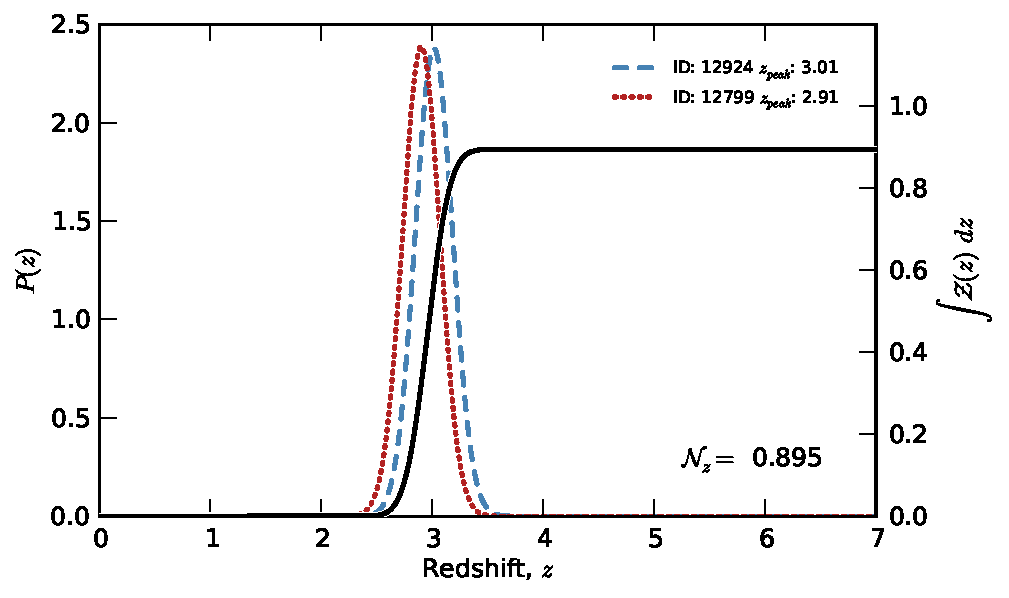
\includegraphics[width=\columnwidth]{plots/PairsPz_pri_81_2.pdf}
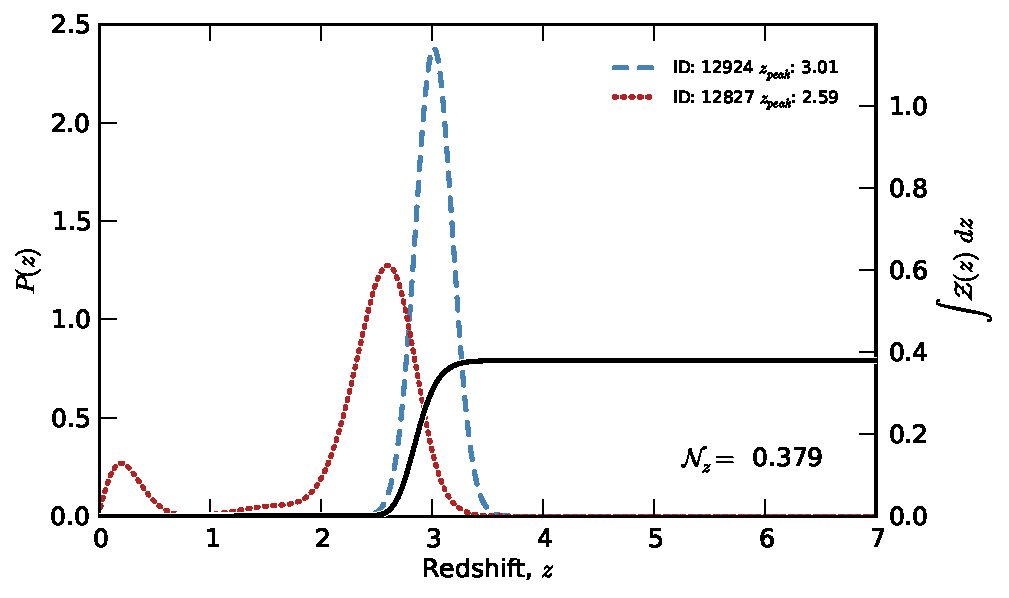
\includegraphics[width=\columnwidth]{plots/PairsPz_pri_81_4.pdf}
  
  \caption[Example redshift PDFs and integrated $\mathcal{Z}(z)$ for two projected pairs around a primary galaxy at $z\approx 3.01$ in the \emph{Hubble} Ultra Deep Field.]{Example redshift PDFs and integrated $\mathcal{Z}(z)$ for two projected pairs around a primary galaxy at $z\approx 3.01$ in the \emph{Hubble} Ultra Deep Field. In both panels, the blue dashed line corresponds to the redshift PDF for the primary galaxy while red the dotted line is that of the projected companion. The solid black line shows the cumulative integrated $\mathcal{Z}(z)$ for the galaxy pair.}
  \label{merger-fig:pairs_pz}
\end{figure}

In Figure~\ref{merger-fig:pairs_pz} we show two examples of projected pairs around a primary galaxy that sits within the Hubble Ultra Deep Field region of CANDELS GOODS South. The primary galaxy sits at $z\approx 3.0$ and has at least one galaxy with a high pair-probability (top panel) and several other companions with a non-negligible pair-probability.

As the redshift probability function takes into account the line-of-sight information for the potential galaxy pair, two additional binary redshift masks are required to enforce the additional pair selection criteria. These masks are equal to one at a given redshift when the selection criteria are satisfied and zero otherwise. As above, we follow the notation outlined in \citetalias{LopezSanjuan:2014uj} and define the angular separation mask, $\mathcal{M}^{\theta}(z)$, as
\begin{equation}
\mathcal{M}^{\theta}(z) = 
\begin{cases}
1, & \text{ if } \theta_{min}(z) \leq \theta \leq \theta_{max}(z) \\ 
0, & \text{ otherwise, } 
\end{cases}
\end{equation}
where the angular separation between the galaxies in a pair as a function of redshift is denoted $\theta (z)$. The angular separation is a function of the projected distance $r_{p}$ and the angular diameter distance, $d_{A}(z)$, for a given redshift and cosmology, i.e. $\theta_{max}(z) = r^{max}_{p} / d_{A}(z)$ and $\theta_{min}(z) = r^{min}_{p} / d_{A}(z)$.

The pair selection mask, denoted $\mathcal{M}^{\rm{pair}}(z)$, is where our method differs to that outlined by \citetalias{LopezSanjuan:2014uj}. Rather than selecting galaxy pairs based on the luminosity ratio, we instead select based on the estimated stellar mass ratio. We define our pair-selection mask as
\begin{equation}\label{eq:sel_mask}
\mathcal{M}^{\rm{pair}}(z) = 
\begin{cases}
1, & \text{ if } \Mstar^{\rm{lim},1}(z) \leq \rm{M}_{\star,1}(z) \leq \rm{M}_{\star,max}  \\ 
	& \text{ and }~ \Mstar^{\rm{lim},2}(z) \leq \rm{M}_{\star,2}(z) \\
0, & \text{ otherwise. } 
\end{cases}
\end{equation}
where $\rm{M}_{\star,1}(z)$ and $\rm{M}_{\star,2}(z)$ are the stellar mass as a function of redshift, details of how $\rm{M}_{\star}(z)$ is calculated for each galaxies are discussed in Section~\ref{merger-sec:stellarmass}. The flux-limited mass cuts, $\Mstar^{\rm{lim},1}(z)$ and $\Mstar^{\rm{lim},2}(z)$, are given by
\begin{equation}\label{eq:fluxlim_pri}
\Mstar^{\rm{lim},1}(z)= max \{ \Mstar^{\rm{min}}, \Mstar^{\rm{flux}}(z) \}
\end{equation}
and
\begin{equation}\label{eq:fluxlim_sec}
\Mstar^{\rm{lim},2}(z) = max \{ \mu \Mstar^{1}(z), \Mstar^{\rm{flux}}(z) \}
\end{equation}
respectively, where $\Mstar^{\rm{flux}}(z)$ is the redshift-dependent mass completeness limit outlined in Section~\ref{merger-sec:weights_flux} and $\Mstar^{min}$ and $\Mstar^{max}$ are the lower and upper ranges of our target sample of interest. The mass ratio $\mu$ is typically defined as $\mu = 1/4$ for major mergers and $\mu = 1/10$ for minor mergers, throughout this work we set $\mu = 1/4$ by default unless otherwise stated. This pair selection mask ensures the following criteria are met at each redshift. Firstly, the primary galaxy is within the mass range of interest. Secondly, the mass ratio between the primary and secondary galaxy is within the desired range (e.g. for selecting major or minor mergers). And finally that both the primary and secondary galaxy are above the mass completeness limit at the corresponding redshift. We note that the first criteria of Equation~\ref{eq:sel_mask} also constitutes the selection function for the primary sample, given by
\begin{equation}\label{eq:pri_sel}
S(z) = 
\begin{cases}
1, & \text{ if } \Mstar^{\rm{lim},1}(z) \leq \rm{M}_{\star,1}(z) \leq \rm{M}_{\star,max}  \\ 
0, & \text{ otherwise. } 
\end{cases}
\end{equation}


With these three properties in hand for each potential companion galaxy around our primary target, the pair-probability function, $\textup{PPF}(z)$, is then given by
\begin{equation}\label{eq:PPF}
\textup{PPF}(z) = \mathcal{Z}(z) \times \mathcal{M}^{\theta}(z) \times \mathcal{M}^{\text{pair}}(z).
\end{equation}
In Section~\ref{merger-sec:pair_frac} we outline how this pair-probability function is integrated to determine the photometric pair-probability, but first we outline how the photometric redshifts and stellar masses used in this analysis were estimated and then outline the steps taken to correct for selection effects within the data.

\subsection{Photometric redshifts}\label{merger-sec:photoz}
Photometric redshifts for all sources are calculated using the \textsc{eazy} photometric redshift code \citep{Brammer:2008gn}. The redshifts were fit to all available photometric bands for each field as outlined in Section~\ref{merger-sec:data} and made use of the default \textsc{eazy} reduced template set plus the addition of a young Ly$\alpha$ emitting galaxy template based on the spectrum of \citet{2010ApJ...719.1168E}. We construct the redshift probability distribution (PDF, $P(z)$) for each galaxy from its $\chi^{2}$ distribution following $P(z) \propto \exp(-\chi^{2}(z)/2)$.

When calculating the galaxy PDFs we do not make use of a luminosity-dependent redshift prior as is commonly done \citep{Brammer:2008gn,Dahlen:2013eu}. Luminosity dependent priors such as the one implemented in \textsc{eazy} rely on model lightcones which accurately reproduce the observed (apparent) luminosity function. Current semi-analytic models do agree well with observations at $z < 2$ \citep{Henriques:2012gsa}, but increasingly diverge at higher redshift.

Furthermore, the use of a prior which is only dependent on a galaxy's luminosity and not its colour or wider SED properties could significantly bias the estimation of close pairs using redshift PDFs. Consider a pair of galaxies at identical redshifts and with identical stellar population properties, where the only difference is the stellar mass of the galaxy (i.e. similar star-formation histories, differing only in normalisation). A luminosity-dependent prior will change the posterior probability distribution for each galaxy individually and could erroneously decrease the integrated pair probability. The effects of luminosity-based priors on redshift PDFs at $z < 3$ where SAMs are much better constrained are explored in further detail in Mundy et al. \emph{in prep}.

As discussed in \citet{Hildebrandt:2008jh} and \citet{Dahlen:2013eu}, the redshift probability density functions output by photometric redshift codes can often be an inaccurate representation of the true photometric redshift error. This inaccuracy can be due to under- or over-estimates of photometric errors, or a result of systematic effects such as the template choices. Whatever the cause, it can result in significantly over or underestimated 1 and 2 $\sigma$ errors whilst still producing good agreement with between the best-fit $z_{\rm{phot}}$ and corresponding $z_{\rm{spec}}$. Although this systematic effect may be negated when measuring the bulk properties of larger galaxies samples, the method outlined in this chapter relies on the direct comparison of individual redshift PDFs so it is essential that they accurately represent the true uncertainties.

We therefore endeavour to ensure the accuracy of our redshift PDFs before undertaking any analysis based on their PDFs. Following the method outlined in \citet{Dahlen:2013eu}, we first calculate the fraction of spectroscopic redshifts which fall inside the corresponding 68.3\% photo-z confidence intervals. Based on the raw PDFs output by EAZY, we find that of 302 galaxies with high-quality spectroscopic redshifts at $z > 2$, only 35 \% fall inside the corresponding 1$\sigma$ PDF confidence intervals, indicating that our redshift errors are being underestimated. We therefore smooth the PDFs using a boxcar filter and recalculate the fraction of spectroscopic redshifts within the 1$\sigma$, repeating until this value reaches 68.3\%.

\begin{figure}
\centering
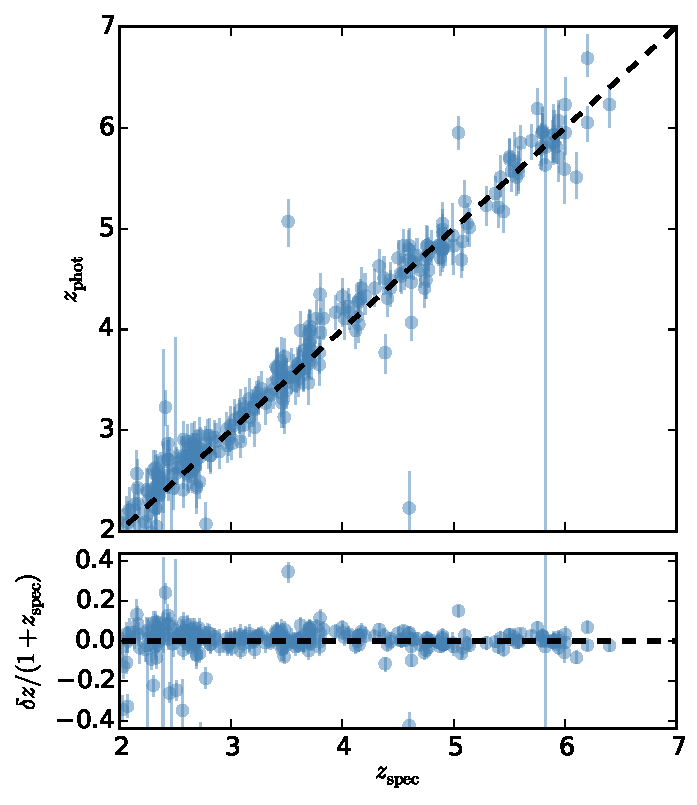
\includegraphics[width=0.85\columnwidth]{plots/specz_comparison.pdf}  
  \caption[Comparison between spectroscopic and photometric redshift for the galaxies in our sample.]{Comparison between spectroscopic and photometric redshift for the galaxies in our sample with available spectroscopy at $z \geq 2$, spectroscopic redshift quality of `Good' or better and apparent magnitude of $H_{160} > 23.5$. The photometric redshift shown is the peak of the probability distribution ($\chi^2$ minimum) with 1-$\sigma$ lower and upper limits after smoothing of $P(z)$ outlined in the text. The bottom panel shows the normalised residuals ($ \Delta z = z_{\text{phot}} - z_{\text{spec}}$) as a function of the measured spectroscopic redshift.}
  \label{merger-fig:specz_comp1}
\end{figure}

In Figure~\ref{merger-fig:specz_comp1} we compare our photometric redshifts and their corrected 1$\sigma$ errors with the available faint spectroscopic redshift samples\footnote{References for the compiled spectroscopic redshift sample can be found in Chapter~\ref{ch:smf}.} ($H_{160} \geq 23.5$). Following the same metrics as in \citet{Molino:2014iz} and \citetalias{LopezSanjuan:2014uj}, we find that the quality of photometric redshifts is excellent given the high-redshifts being studied and the broadband nature of the photometry catalog. We find a normalised median absolute deviation\footnote{The normalised median absolute deviation is defined as $\sigma_{\text{NMAD}} = 1.48 \times \rm{median} \left (  \frac{\left | \Delta z \right |}{1+z_{\rm{spec}}} \right )$, see \citet{Dahlen:2013eu}.} of $\sigma_{\text{NMAD}} = 0.036$ and a bias of $\text{median}(z_{\rm{phot}} - z_{\rm{spec}}) = 0.03$.

As acknowledged in Chapter~\ref{ch:smf}, the typically bright nature of the galaxies with high quality spectroscopic redshift may present a biased representation of the quality of the photometric redshifts. The selection of only the fainter sources with spectroscopic redshifts ($H_{160} \geq 23.5$) is designed to minimise this potential bias. We are also confident that the photometric redshift accuracy fainter galaxies remains high based on the results of the photometric redshift analysis performed on mock galaxies simulations in Chapter~\ref{ch:smf}.

\subsection{Stellar mass estimation}\label{merger-sec:stellarmass}
The stellar mass as a function of redshift, $\textup{M}_{*} (z)$, for each galaxy is estimated using a modified version of the SED code introduced in Chapter~\ref{ch:smf} to which we refer the reader for further details. Rather than estimating the best-fit mass (or mass likelihood distribution) for a fixed input photometric or spectroscopic redshift, we instead estimate the stellar mass at all redshifts in the photometric redshift fitting range simultaneously. Specifically, we calculate the likelihood-weighted mean:
\begin{equation}
	\textup{M}_{*} (z) = \frac{\sum_{t}^{} w_{t}(z) \text{M}_{*,t}(z)} {\sum_{t} w_{t}(z)}
\end{equation}
where the sum is over all galaxy template types, $t$, with ages less than the age of the Universe at the redshift $z$ and $\textup{M}_{\star,t}(z)$ is the optimum stellar mass for each galaxy template (Equation~\ref{eq:temp_norm}). The likelihood, $w_{t}(z)$, is determined by
\begin{equation}
	w_{t}(z) = \exp(-\chi_{t}^{2}(z)/2),	
\end{equation}
where $\chi^{2}_{t}(z)$ is given by:
\begin{equation}\label{eqn:chi}
  \chi^{2}_{t}(z) = \sum_{j}^{N_{filters}} \frac{(\textup{M}_{\star,t}(z) F_{j,t}(z) - F_{j}^{obs})^2} {\sigma_{j}^{2}}.
\end{equation}
The sum is over $j$ filters available for each galaxy, its observed photometric fluxes, $F_{j}^{\textup{obs}}$ and corresponding error, $\sigma_{j}$. The optimum scaling for each galaxy template type (each normalised to 1 M$_{\odot}$), $\textup{M}_{\star,t}$, is calculated analytically by setting the differential of Equation~\ref{eqn:chi} equal to 0 and rearranging to give:
\begin{equation}\label{eq:temp_norm}
	\textup{M}_{\star,t}(z) = 
\frac{\sum_{j} \frac{F_{j,t}(z)F_{j}^{obs}}{\sigma^{2}_{j}} }  { \sum_{j} \frac{F_{j,t}(z)^{2}}{\sigma^{2}_{j}}  }.
\end{equation}
In this work we also incorporate a so-called ``template error function" to account for uncertainties caused by the limited template set and any potential systematic offsets as a function of wavelength. The template error function and method applied to our stellar mass fits is identical to that outlined in \citet{Brammer:2008gn} and included in the initial photometric redshift analysis outlined in Section~\ref{merger-sec:photoz}. Specifically, this means that the total error for any individual filter, $j$, is given by:
\begin{equation}
	\sigma_{j} = \sqrt{\sigma_{j,obs}^{2} + \left ( F_{j,obs}\sigma_{\textup{temp}}(\lambda_{j}) \right )^{2} }
\end{equation}
where $\sigma_{j,obs}$ is observed photometric flux error, $F_{j,obs}$ its corresponding flux and $\sigma_{\textup{temp}}(\lambda_{j})$ the template error function interpolated at the pivot wavelength for that filter, $\lambda_{j}$. We note that in addition to estimating the stellar mass, this method also provides a secondary measurement of the photometric redshift, whereby \(P(z) \propto \sum_{t} w_{t}(z) \). Our reasons for using an independently estimated redshift PDF in the pair analysis in place of those generated by the marginalised redshift likelihoods from the stellar mass fits are two-fold. Firstly, for consistency with results of Chapter~\ref{ch:smf} where the redshifts from \textsc{eazy} have been well tested at high-redshift. And secondly, the fact that the accuracy and reliability offered by \textsc{eazy} is greater due to its ability to fit non-negative combinations of multiple templates simultaneously \citep{Brammer:2008gn,Dahlen:2013eu}.

For the \citet{Bruzual:2003ckb} templates used in our stellar mass fitting we allow a similar range of stellar population parameters as used in Chapter~\ref{ch:smf}. Model ages are allowed to vary from 10 Myr to the age of the Universe at a given redshift, metallicities of 0.02, 0.2 and 1 Z$_{\odot}$, and dust attenuation strength in the range $0 \le A_{V} \le 3$ assuming a \citet{2000ApJ...533..682C} attenuation curve. The assumed star-formation histories follow exponential $\tau$-models ($SFR \propto e^{-t/\tau}$), both decreasing and increasing (negative $\tau$), for characteristic timescales of $\left | \tau \right | = $ 0.25, 0.5, 1, 2.5, 5, 10, plus an additional short burst ($\tau = 0.05$) and continuous star-formation models ($\tau \gg1/H_{0}$). 

Nebular emission is included assuming a relatively high escape fraction $f_{\text{esc}} = 0.2$ \citep{Yajima:2010fb,Fernandez:2011cw,Finkelstein:2012hr,Robertson:2013ji} and hence a relatively conservative estimate on the contribution of nebular emission. As in Chapter~\ref{ch:smf}, we assume for the nebular emission that the gas-phase stellar metallicities are equivalent and that stellar and nebular emission are attenuated by dust equally.

\begin{figure}
\centering
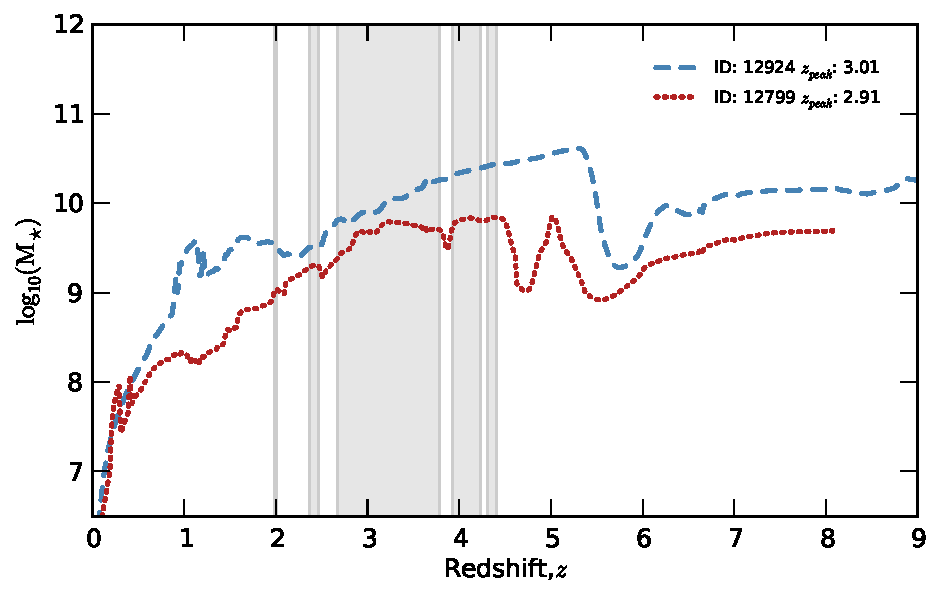
\includegraphics[width=0.9\columnwidth]{plots/PairsMass_pri_81_2.pdf}
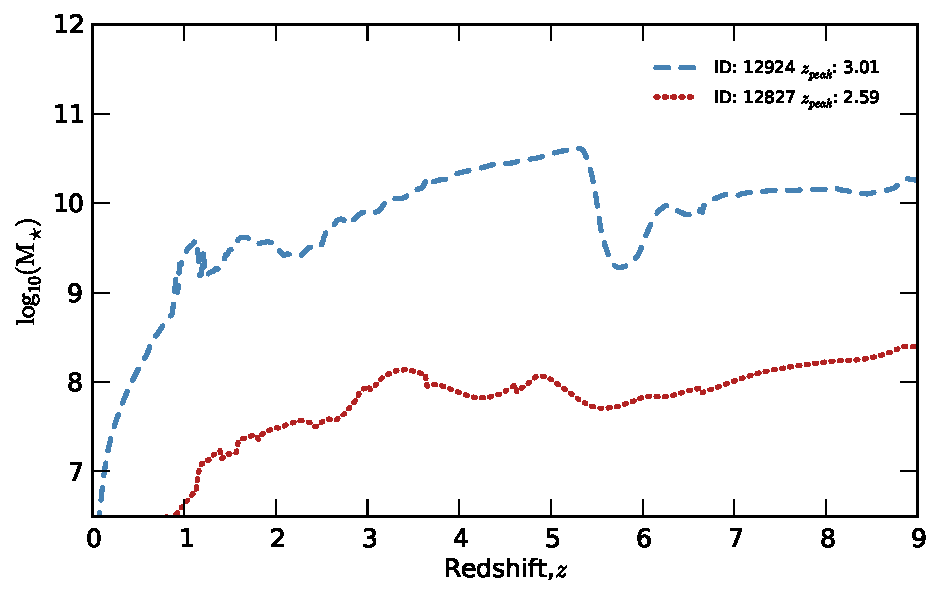
\includegraphics[width=0.9\columnwidth]{plots/PairsMass_pri_81_4.pdf}
  
  \caption[redshift-dependent stellar mass estimations for the example close pairs shown in Figure~\ref{merger-fig:pairs_pz}.]{redshift-dependent stellar mass estimations for the example close pairs shown in Figure~\ref{merger-fig:pairs_pz}. In both panels, the blue dashed line corresponds to the stellar mass for the primary galaxy while the red dotted line is that of the projected companion. The grey shaded regions highlight the redshift ranges in which the pair-selection criteria are met (Equation~\ref{eq:sel_mask}), with $\log_{10}(\Mstar^{min}) = 9.5$ and $\mu = 1/4$.}
  \label{merger-fig:pairs_mass}
\end{figure}

In Figure~\ref{merger-fig:pairs_mass}, we show the estimated stellar mass as a function of redshift for the two example projected pairs shown in Figure~\ref{merger-fig:pairs_pz}. For the galaxy pair shown in the top panel (with $\mathcal{N}_{z} = 0.895$) the pair selection criteria are all satisfied over most of the redshift range with high probability ($z\sim3$). As this pair also satisfies the separation criteria, the pair-probability for this projected pair is $\int_{0}^{\infty} \textup{PPF}(z) dz = 0.869$. In contrast, the second potential pair (with $\mathcal{N}_{z} = 0.379$) does not satisfy the pair criteria at any redshift due to the low stellar mass of the secondary galaxy and therefore has a final pair-probability of $\int_{0}^{\infty} \textup{PPF}(z) dz = 0.$.

\subsection{Correction for selection effects}
As defined by \citetalias{LopezSanjuan:2014uj}, the pair-probability function in Equation~\ref{eq:PPF} is affected by two selection effects. Firstly, the incompleteness in search area around galaxies that are near the image boundaries or near areas affected by bright stars (Section~\ref{merger-sec:weights_area}). And secondly, the selection in photometric redshift quality (Section~\ref{merger-sec:weights_osr}). Additionally, because in this work we use a flux-limited sample rather than one that is volume limited (as used by \citetalias{LopezSanjuan:2014uj}), we must also include a further correction to account for this fact.

\subsubsection{The redshift-dependent mass completeness limit}\label{merger-sec:weights_flux}
Since the photometric survey we are using includes regions of different depth and high-redshift galaxies are by their very nature quite faint, restricting our analysis to a volume-limited sample would necessitate excluding the vast majority of the available data. As such, we choose to use a redshift-dependent mass completeness limit with the limit determined by the flux limit determined by the survey. 

Due to the limited number of galaxy sources available, determining the strict mass completeness as a function of redshift entirely empirically \citep{Pozzetti:2010gw} is not possible. Instead, we make use of a semi-empirical method based on that of \citet{Pozzetti:2010gw}, using the available observed stellar mass estimates to inform the selection of a template SED for the evolving 95\% stellar mass-to-light limit. We make use of the full set of high-redshift Monte Carlo samples of Chapter~\ref{ch:smf}, selecting galaxies which are within a given redshift bin, then scaling the masses of the faintest 20\% such that their apparent magnitude is equal to the flux limit. The mass completeness limit for a given redshift bin is defined as the mass corresponding to the 95th percentile of the scaled mass range, the resulting mass completeness at $z > 3.5$ in bins with width $\Delta z = 0.5$ are shown in Figure~\ref{merger-fig:mass_comp} assuming a flux-limit equal to that in the GOODS South `DEEP' region.

\begin{figure}
\centering
	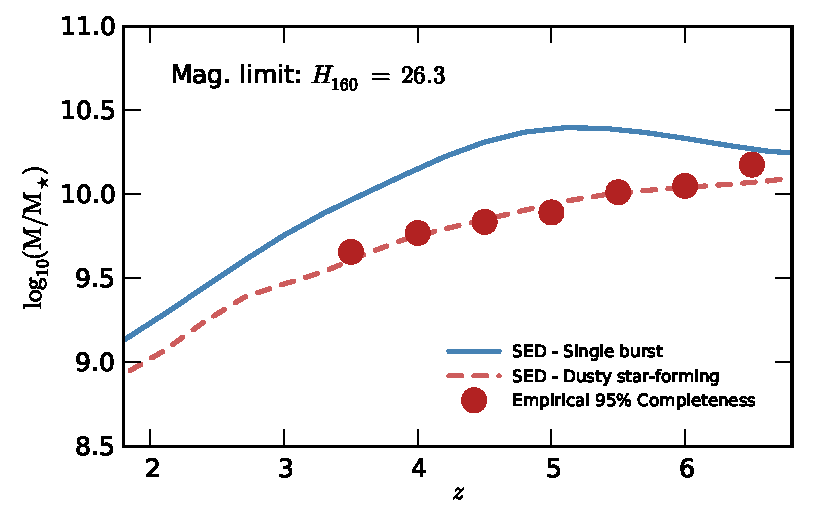
\includegraphics[width=0.8\columnwidth]{plots/MassCompleteness.pdf}
  \caption[]{Mass completeness limit corresponding to a flux limit of $H_{160} = 26.3$, the approximate depth of the DEEP and ERS regions within CANDELS GOODS South. Red circles correspond to the 95\% completeness limits derived from the stellar mass estimates of Chapter~\ref{ch:smf}, the continuous blue and dashed red lines are the completeness limits corresponding to a maximally old (at a given redshift) single burst or dusty star-forming population respectively, see text for details.}
  \label{merger-fig:mass_comp}
\end{figure}

Based on the estimated completeness limits, we select a \citet{Bruzual:2003ckb} template that closely matches the observed $\Mstar/\textit{L}$ redshift evolution. By doing so we can estimate the mass completeness as a continuous function of redshift and extend the constraints to redshifts lower than those explored in Chapter~\ref{ch:smf}. A common choice of template for estimating the strict $\Mstar/\textit{L}$ completeness is a maximally old single burst (continuous blue line in Figure~\ref{merger-fig:mass_comp}). However, since the vast majority of galaxies above $z\sim3$ are star-forming, this assumption significantly overestimates the actual completeness limit at high-redshift. Based on plausible assumptions for galaxies at high-redshift and tuning by hand, we find a maximally old, very dusty ($A_{V} = 2$) star-forming galaxy with a power-law star-formation history ($\propto t^{1.4}$) provides a good fit to the empirical data (red dashed line in Figure~\ref{merger-fig:mass_comp}). For both the burst and star-forming SEDs, we assume an onset of star-formation at $z = 12$, sub-solar metallicity (0.2 $Z_{\odot}$) and an escape fraction for nebular emission of $f_{\rm{esc}} = 0.2$. 

While a dust extinction of $A_{V} = 2$ is higher than typically observed at high redshift \citep{2015A&A...574A..19S}, it is consistent with the dust extinction seen in sub-mm galaxies at $z > 2$ \citep{Targett:2013kg,Wiklind:2014gs,Smolcic:2015ke} and therefore represents a plausible limit for the highest mass-to-light ratios at high redshift. Instead of assuming a rising star-formation history and high fixed dust attenuation, we could have instead plausibly chosen a different star-formation history and allowed dust to vary with redshift in a manner which also matched the estimated empirical completeness.

The redshift-dependent mass limit, $\Mstar^{\rm{flux}}(z)$, is defined as
\begin{equation}\label{eq:fluxlim}
	\log_{10}(\Mstar^{\rm{flux}}(z)) = 	0.4\times( H_{\Mstar/\textit{L}}(z) - H^{\rm{lim}})
\end{equation}
where $H^{\rm{lim}}$ is the $H_{160}$ magnitude at the flux-completeness limit in the field or region of interest and $H_{\Mstar/\textit{L}}(z)$ is the $H_{160}$ magnitude of the dusty star-forming template normalised to 1 $\rm{M}_{\odot}$ and observed through the $H_{160}$ at a given redshift (automatically taking the required $k$-correction into account).

For a primary galaxy with a mass close to the redshift-dependent mass-limit imposed by the selection criteria $S(z)$, the mass range within which secondary pairs can included may be reduced, i.e.  $\mu\Mstar^{1}(z) <  \Mstar^{\rm{lim}}(z) < \Mstar^{1}(z)$. To correct for the potential galaxy pairs that may be lost by the applied completeness limit, we make a statistical correction based on the stellar mass function at the redshift of interest. The flux-limit weight, $w^{\text{flux}}_{2}(z)$, applied to every secondary galaxy found around each primary galaxy, is defined as 
\begin{equation}
	w^{\text{flux}}_{2}(z) = \frac{1} {W_{2}(z)},	
\end{equation}
where 
\begin{equation}
	W_{2}(z) = \frac{ \int_{\Mstar^{\text{lim}}(z)}^{\Mstar^{\text{1}}(z)} 
								\phi(\Mstar|z)d\Mstar} 
								{ \int_{\mu \Mstar^{1}(z)}^{\Mstar^{\text{1}}(z)}
								\phi(\Mstar|z)d\Mstar}
\end{equation}
and \( \phi(\Mstar|z) \) is the stellar mass function at the corresponding redshift. The redshift-dependent mass limit is \(\Mstar^{\text{lim}}(z) = max \{ \mu \Mstar^{1}(z), \Mstar^{\rm{flux}}(z) \} \), where \(\Mstar^{\rm{flux}}(z)\) is defined in Equation~\ref{eq:fluxlim}). By applying this weight to all pairs associated with a primary galaxy, we get the the pair statistics corresponding to $\mu \Mstar^{1}(z) \leq \Mstar^{\text{2}}(z) \leq \Mstar^{\text{1}}(z)$ (the volume limited case). As in \citet{Patton:2000kt}, we assign additional weights to the primary sample in order to minimise the error from primary galaxies that are closer to the flux limit (i.e. PDF weighted to higher redshifts) as these galaxies will have fewer numbers of \emph{observed} pairs. The primary flux-weight, $w_{\text{flux}}^{1}(z)$ is defined as
\begin{equation}
	w^{\text{flux}}_{1}(z) =  W_{1}(z) = \frac{ \int_{\Mstar^{\text{lim}}(z)}^{\Mstar^{\rm{max}}} 
																	\phi(\Mstar|z)d\Mstar} { \int_{\Mstar^{\rm{min}}}^{\Mstar^{\rm{max}}}
																	\phi(\Mstar|z)d\Mstar}
\end{equation}
where $\Mstar^{\rm{min}}$ and $\Mstar^{\rm{max}}$ are the lower and upper limits of the mass range of interest for the primary galaxy sample, the redshift-dependent lower limit is defined as \( \Mstar^{\text{lim}}(z) = max \{ \Mstar^{\rm{min}}, \Mstar^{\rm{flux}}(z) \} \), and the remaining parameters are as outlined above. In the case of a volume-limited sample (where \(\Mstar^{\rm{flux}}(z) < \mu\Mstar^{1}(z) \) at all redshifts) both of the flux-limit weights are equal to unity.

The stellar mass functions (SMF) parametrisations as a function of redshift, \( \phi(\Mstar|z) \), are taken from \citet{Mortlock:2014et} at $z \leq 3$, \citet{Santini:2012jq} at $3 < z < 3.5$ and Chapter~\ref{ch:smf} at $z \geq 3.5$. When selecting redshift bins in which to estimate the merger fraction, we ensure that the bins are chosen to match the bins in which the SMF are constrained (i.e. the SMF used to weight the merger fraction is the same across the bin).

To calculate the effective completeness weights for comparison requires integrating over the redshift dependent $w^{\text{flux}}_{1}(z)$ or $w^{\text{flux}}_{2}(z)$. When doing so we must also take into account the redshifts at which the primary and secondary galaxy are contributing to the total galaxy pair count and therefore the redshifts at which the completeness weights are being applied. As such, we define the pair-weighted flux completeness weights for a galaxy pair, $\left \langle w^{\text{flux}}_{n} \right \rangle ^{i,j}$, as
\begin{equation}
	\left \langle w^{\text{flux}}_{n} \right \rangle^{i,j} = \frac{\int \text{PPF}^{i,j}(z) w^{\text{flux, i}}_{n}(z) \text{d}z}{\int \text{PPF}^{i,j}(z) \text{d}z},
\end{equation}
where $n$ equals either 1 or 2, corresponding to the primary or secondary flux-weight respectively. Similarly, $i$ and $j$ are the primary and secondary galaxies in a galaxy pair, with  $\text{PPF}^{i,j}(z)$ the corresponding pair probability function. 

\begin{figure*}
\centering
	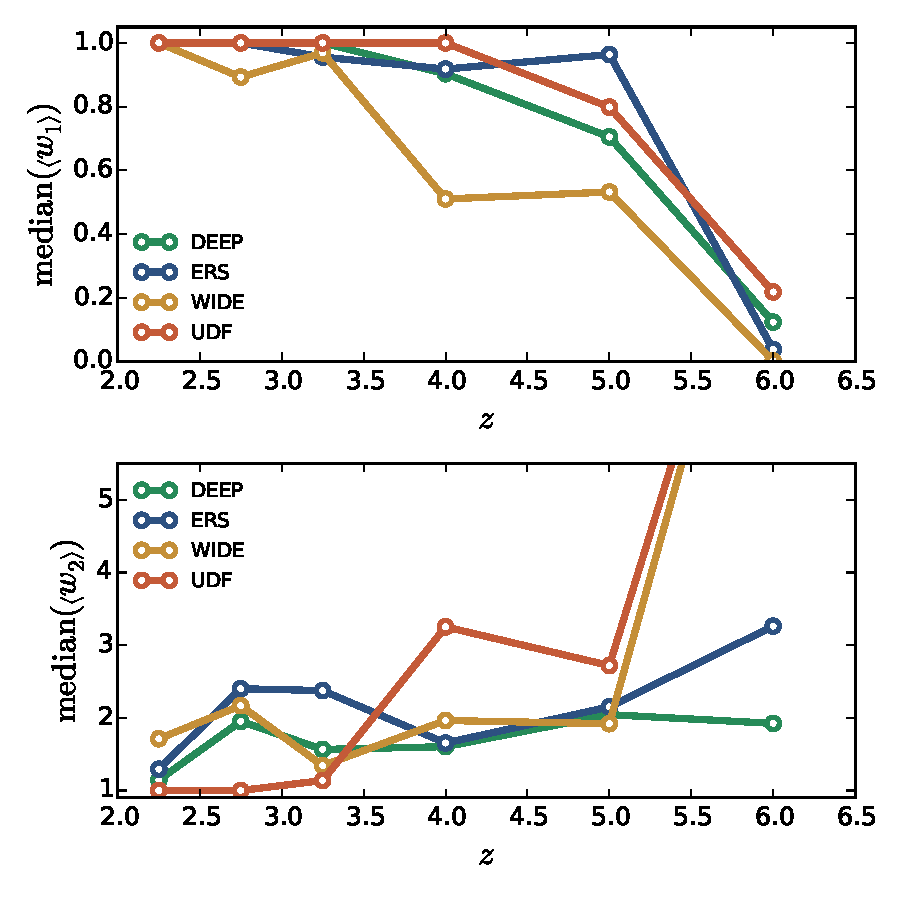
\includegraphics[width=0.85\columnwidth]{plots/flux_weight_means_MCtests.pdf}
  \caption[The median completeness weights as a function of redshift for each region of GOODS South.]{The median completeness weights as a function of redshift for each region of GOODS South, assuming a mass selection of $\log_{10}(\Mstar / \text{M}_{\odot}) > 9.5$ and minimum mass ratio of $\mu = \frac{1}{4}$.}
  \label{merger-fig:flux_weights_medians}
\end{figure*}

To see how the the completeness weights change as a function of redshift and limiting depth (i.e. the variation between regions in GOODS South) we calculated the median completeness weights in each of the redshift bins used later in Section~\ref{merger-sec:mergerfraction} and \ref{merger-sec:mergerrate}. The resulting completeness weights for each region of GOODS South are shown in Figure~\ref{merger-fig:flux_weights_medians}, assuming a mass selection of $\log_{10}(\Mstar / \text{M}_{\odot}) > 9.5$ and minimum mass ratio of $\mu = \frac{1}{4}$ when calculating $\text{PPF}^{i,j}(z)$. As $\log_{10}(\Mstar / \text{M}_{\odot}) > 9.5$ is the lowest mass limit used in this work, the pair-weighted completeness weights shown in Figure~\ref{merger-fig:flux_weights_medians} represent the lower or upper limits for the primary and secondary weights respectively.

In addition to the median pair-weighted completeness weights, we also estimated the effects of the errors in the stellar mass function parametrizations as a function of redshift. We estimated the errors by randomly perturbing the Schechter function parameters in each redshift bin by their quoted errors and then re-calculating $\left \langle w^{\text{flux}}_{n} \right \rangle$, repeating this process 32 times to give a distribution of pair-weighted completeness weights for each individual galaxy pair. In Figure~\ref{merger-fig:flux_weights_errs} we show the average fractional standard deviation in each redshift bin for both the primary and secondary completeness weights.

\begin{figure*}
\centering
	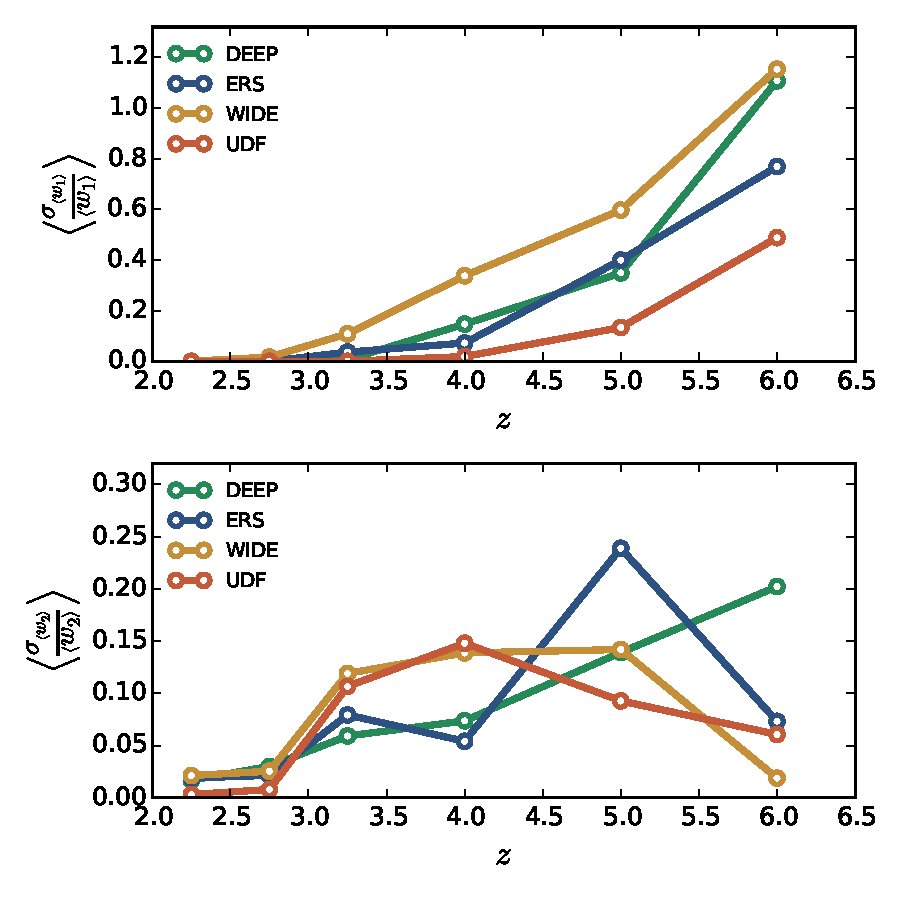
\includegraphics[width=0.85\columnwidth]{plots/flux_weight_MCtests.pdf}
  \caption[Effect of stellar mass function errors on $w_{1}$ and $w_{2}$.]{Effect of stellar mass function errors on $w_{1}$ and $w_{2}$.}
  \label{merger-fig:flux_weights_errs}
\end{figure*}

Inspecting Figures~\ref{merger-fig:flux_weights_medians} and \ref{merger-fig:flux_weights_errs}, we find that up to $z\sim4$, the completeness weights remain relatively small and have low errors due to the uncertainties in the observed stellar mass functions. However at $z\gtrsim4$, the weights become increasingly large ($\text{median} (\left \langle w^{\text{flux}}_{2} \right \rangle)$) or have much greater uncertainty ($\sigma_{\left \langle w^{\text{flux}}_{1} \right \rangle}$). These results suggest that for redshifts $z \geq 5$, the mass completeness corrections become increasingly important, but also that they will be increasingly unreliable. As such, these uncertainties will likely place an upper limit on the redshifts at which we can estimate the major merger rate. 

\subsubsection{Image boundary and excluded regions}\label{merger-sec:weights_area}
A second correction which must be taken into account is to the search area around primary galaxies that lie close to the boundaries of the survey region. Because of the fixed physical search distance, this correction is also a function of redshift so must be calculated for all redshifts within the range of interest.

In addition to the area lost at the survey boundaries, it is also necessary to correct for the potential search area lost due to the presence of large stars and other artefacts, around which no sources are included in the catalog (see Section~\ref{merger-sec:initial}). 

We have taken both of these effects into account when correcting for the search areas by creating a mask image based on the underlying photometry. Firstly, we define the image boundary based on the exposure map corresponding to the $H_{160}$ photometry used for object detection. Next, for every source excluded from the sample catalog based its classification as a star or image artefact by our photometric or visual classification, the area corresponding to that object (from the photometry segmentation map) is set to zero in our mask image. Finally, areas of photometry which are labelled in the flag map (and excluded based on their corresponding catalog flags) are also set to zero.

To calculate the area around a primary galaxy that is excluded by these effects, we perform photometry on the mask image.  Photometry is performed in annuli around each primary galaxy target, with inner and outer radii of $\theta_{\rm{min}}(z)$ and $\theta_{\rm{max}}(z)$ respectively. The area weight is then defined as
\begin{equation}
	w_{\rm{area}}(z) = \frac{1} {f_{	\rm{area}}(z)}
\end{equation}
where $f_{	\rm{area}}(z)$ is the sum of the normalised mask image within the annulus at a given redshift divided by the sum over the same area in an image with all values equal to unity. By measuring the area in this way we are able to automatically take into account the irregular survey shape and any small calculation errors from quantisation of areas due to finite pixel size.

Despite the relatively small survey area explored in this study (and hence a higher proportion of galaxies likely to lie near the image edge), the effect of the area weight on the estimated pair fractions is very small. To quantify this, we calculate the pair averaged area weights, $\left \langle w_{\rm{area}} \right \rangle$, following the same formalism as outlined for the mass completeness weights above:
\begin{equation}
	\left \langle w_{\rm{area}}^{i,j} \right \rangle = \frac{\int \text{PPF}^{i,j}(z) w_{\rm{area}}^{i}(z) \rm{d}z}{\int \text{PPF}^{i,j}(z) \rm{d}z},
\end{equation}
where $w_{\rm{area}}^{i}(z)$ is the redshift dependent area weight for a primary galaxy $i$, and $\text{PPF}^{i,j}(z)$ the corresponding pair-probability function for primary galaxy and a secondary galaxy $j$. Of the full sample of primary galaxies, less than $10\%$ have average area weights greater than $1\%$ (where a primary galaxy has multiple pairs, we take the average of $\left \langle w_{\rm{area}}^{i,j} \right \rangle$ over all secondary galaxies). Furthermore, only $\approx 2\%$ of primary galaxies have average weights $>10\%$ (i.e. $\left \langle w_{\rm{area}}^{i,j} \right \rangle > 1.1$) and only $0.15\%$ have weights $>50\%$. The effects of area weights on the final estimated merger fractions will therefore be minimal. Never the less, we include these corrections in all subsequent analysis.

\subsubsection{The Odds sampling rate}\label{merger-sec:weights_osr}
Following \citetalias{LopezSanjuan:2014uj}, we also apply a selection based on the photometric redshift quality, or odds $\mathcal{O}$ parameter. The odds parameter is defined by \citet{Benitez:2000jr} and \citet{Molino:2014iz} as
\begin{equation}
	\mathcal{O} = \int_{-K(1+z_{\rm{p}})}^{+K(1+z_{\rm{p}})} P(z) dz
\end{equation}
where $z_{\rm{p}}$ is the redshift corresponding peak of the redshift PDF, $P(z)$ (or the PDF average or median). In \citet{Molino:2014iz} $K = 0.0125$, based on the typical photometric redshift accuracy of their survey. However due to the high redshifts of interest and the broadband nature of the CANDELS survey (as opposed to the lower redshift narrow-band ALHAMBRA survey studied in \citet{Molino:2014iz}) we assume a broader criteria of $K = 0.05$ based on difference in photometric redshift scatter between the two surveys ($\approx 4\times$).

The odds sampling rate (OSR) for galaxies with an apparent $H_{160}$ magnitude of $M$ is then defined as
\begin{equation}
	\text{OSR}(M) = \frac{\sum_{i} N_{i, \mathcal{O} \geq 0.3}} {\sum_{i} N_{i, \mathcal{O} \geq 0} },
\end{equation}
the ratio between the number of galaxies with $\mathcal{O} \geq 0.3$  and the total number of galaxies ($\mathcal{O} \geq 0$) with magnitude $M$ \citep{Molino:2014iz}.

We first calculate $\text{OSR}(M)$ in bins with width $\Delta M = 0.5$ and interpolate these values to define the odds sampling rate for each galaxy based on its apparent $H_{160}$ magnitude. From this value, the OSR weight for each individual galaxy, $i$, is then defined as
\begin{equation}
	w^{\text{OSR}}_{i} = \frac{1} {\text{OSR}(M_{i})}	.
\end{equation}

For both $w^{\text{OSR}}_{1}$ and $w^{\text{OSR}}_{2}$, the average value is $\approx 1.5$ (again, weighted by the corresponding pair likelihoods) and the largest OSR weight is less than 1.8.

\subsubsection{The combined weights}
Taking all three of the above effects into account, the pair weights for each secondary galaxy found around a galaxy primary are given by
\begin{equation}\label{eq:flux_weights_2}
w_{\text{2}}(z) = w^{\text{area}}_{1}(z) \times 
							w^{\text{flux}}_{1}(z) \times w^{\text{flux}}_{2}(z) \times w^{\text{OSR}}_{1}
							\times w^{\text{OSR}}_{2}.
\end{equation}
The weights applied to every primary galaxy in the sample are then given by
\begin{equation}\label{eq:flux_weights_1}
w_{\text{1}} =  w^{\text{flux}}_{1}(z)  \times w^{\text{OSR}}_{1}.
\end{equation}
These weights are then applied to the integrated pair-probability functions for each set of potential pairs to calculate the merger fraction.
As discussed in the previous sections, the greatest contribution to the total weights primarily comes from the secondary galaxy completeness weights, $w^{\text{flux}}_{2}(z)$, with additional non-negligible contributions from the primary completeness and the odds sampling rate weights. Furthermore, the largest error in the total weights results from the mass completeness weights. 

In the implementation of the pair-count methodology used in this chapter, it is not currently possible to fully incorporate the individual completeness weight errors in the overall merger fraction uncertainties. However, in future studies incorporating the full CANDELS datasets where Poisson and cosmic variance errors will be significantly reduced, propagating the SMF uncertainty into the final of increasing importance. For the results presented later in this chapter, it is necessary to bear in mind that there may additional statistical errors in the measured pair-fraction up to $\sigma_{x}/x \lesssim 0.2$.

\subsection{The merger fraction}\label{merger-sec:pair_frac}
For each galaxy, $i$, in the primary sample, the number of associated pairs, $N_{\rm{pair}}^{i}$, within the redshift range $z_{\rm{min}} < z < z_{\rm{max}}$ is given by
\begin{equation}
N_{\text{pair}}^{i} = \sum_{j} \int_{z_{\rm{min}}}^{z_{\rm{max}}} w_{\text{2}}^{j}(z)\times \text{PPF}_{j}(z) dz	
\end{equation}
where $j$ indexes the number of potential close pairs found around the primary galaxy, $\text{PPF}_{j}(z)$ the corresponding pair-probability function (Section~\ref{merger-sec:ppf}) and $w_{\text{2}}^{j}(z)$ its pair weight (Equation~\ref{eq:flux_weights_2}). The corresponding weighted primary galaxy contribution, $N_{1}^{i}$, within the redshift bin is
\begin{equation}
 N_{1}^{i} = \sum_{i}\int_{z_{\rm{min}}}^{z_{\rm{max}}} w_{1}^{i}(z) \times P_{i}(z) \times S_{1}^{i}(z){} dz	
\end{equation} 
where $S_{1}^{i}(z)$ is the selection function for the primary galaxies given in Equation~\ref{eq:pri_sel}, $P_{i}(z)$ its normalised redshift probability distribution and $w_{1}^{i}$ its weighting. In the case of a primary galaxy with stellar mass in the desired range with its redshift PDF contained entirely within the redshift range of interest, $N_{1}^{i} = w_{1}^{i}$ and hence always equal or greater than unity.

The estimated merger fraction $f_{\rm{m}}$ is defined as the number of pairs divided by the total number of galaxies. In the redshift range $z_{\rm{min}} < z < z_{\rm{max}}$,  $f_{\rm{m}}$ is then given by 
\begin{equation}
f_{\rm{m}} = \frac{\sum_{i} N_{\text{pair}}^{i}}{\sum_{i} N_{1}^{i}}
\end{equation}
where $i$ is summed over all galaxies in the primary sample. In the case of a field consisting of different sub-fields with differing depths like GOODS South, this sum becomes 
\begin{equation}
f_{\rm{m}} = \frac{\sum_{k}\sum_{i} N_{\text{pair}}^{k,i}}{\sum_{k}\sum_{i} N_{1}^{k,i}}
\end{equation}
where $k$ is indexed over the number distinct regions within a field (in the case of GOODS South -- Deep, Wide, ERS and UDF) and the flux-limited mass completeness used throughout the calculations is set by the corresponding $H_{160}$ depth within each field.


\section{The merger evolution at $z > 2$}\label{merger-sec:results}
 
For this work we select our initial sample of galaxies in each field based on the following criteria:
\begin{equation}
	\int_{2}^{\infty} P(z)~dz > 0.95, 
\end{equation}
ensuring that the bulk of the redshift probability distribution lies at high redshift and that any secondary redshift solutions are minor. The result of this criteria is to decrease the scatter ($\sigma_{\text{NMAD}} = 0.03$) and bias ($\text{median}(z_{\rm{phot}} - z_{\rm{spec}}) = 0.01$) and give a primary sample with very low outlier fraction. Specifically, for the definitions of outlier fraction in \citet{Molino:2014iz}, we find $\eta_{1} = 0.7\%$ and $\eta_{2} = 1.1\%$.

For this clean high-redshift sample, we then performed the PDF pair-count analysis in six redshift bins from $z = 2$ to $z = 6.5$ for stellar mass cuts of $\log_{10}(\Mstar / \text{M}_{\odot}) > 9.5$ and $\log_{10}(\Mstar / \text{M}_{\odot}) > 10$. We perform the pair searches in two annuli with projected separation $5 \leq r_{\text{p}} \leq 20$ and $5 \leq r_{\text{p}} \leq 30$. The minimum radius of 5 kpc is typically included in close pair analysis to prevent confusion of close sources due to the photometric or spectroscopic fibre resolution. Although the high-resolution HST photometry allows for reliable de-confusion at radii smaller than this \citep{Laidler:2007iy,Galametz:2013dd}, we adopt this radius for consistency with previous results.

The error on $f_\text{m}$ is estimated using the common bootstrap technique of \citet{Efron:1979uf,EFRON:HJ2mD4hg}. The standard error, $\sigma_{f_{\text{m}}}$, is defined as
\begin{equation}\label{eq:bootstrap_err}
	\sigma_{f_{\rm{M}}} = 
	\sqrt{\frac{\sum_{i}^{N} \left (f_{\text{m}}^{i} - \left \langle f_{\text{m}}  \right \rangle \right)^{2}}
	{(N-1)}
	} 
\end{equation}
where $f_{\text{m}}^{i}$ is the estimated merger fraction for a randomly drawn sample of galaxies (with replacement) from the initial sample (for $N$ independent realisations) and $\left \langle f_{\text{m}} \right \rangle =  \left( \sum_{i} f_{\text{m}}^{i} \right) / N $. The results of this analysis are outlined in Section~\ref{merger-sec:mergerfraction}.

\subsection{Merger fractions for semi-analytical models}
To make a direct comparison with theoretical models we also perform the pair-count analysis on mock lightcones from the semi-analytical models (SAMs) of \citeauthor{Lu:2011hj} (\citeyear{Lu:2011hj}, see also \citeauthor{Lu:2014kl}~\citeyear{Lu:2014kl}). We treat the mock data as a `perfect' spectroscopic survey and apply a pseudo-spectroscopic pair-count methodology for the same separation and mass criteria as used on the observational data, using a separation criteria of $\Delta v \leq 500~\rm{km~s}^{-1}$ along the line-of-sight.

Although the field size of the lightcone is approximately $10\times$ the size of the observed GOODS South field, the counts obtained are still subject to significant errors due to cosmic variance. To minimise the effects of cosmic variance, we apply the analysis to 8 different realisations of the mock lightcone, taking the average and standard deviation of these values. We calculate the pair-counts for overlapping redshift bins with width $\Delta z = 0.5$, in steps of half this size. Due to volume limitations at low-redshift and the simulation time and resolution limits at high-redshift, we restrict the mock pair-count analysis to $0.5 \leq z \leq 5.75$.

\subsubsection{Cosmic variance estimates from SAMs}\label{merger-sec:CV_SAM}
The large field size of the SAMs and the multiple realisations of the lightcone (effectively simulating separate fields on the sky) also allows us to make well informed estimates of the cosmic variance (CV) for our observations. We estimate the CV error for the GOODS South field by repeatedly measuring the pair-counts in the mock lightcones using a field size equal to that of the CANDELS field ($10 \times 16 ~ \text{arcmin}$). The position of the sub-region being studied is selected randomly from five of the lightcones and centred at a random position within the larger lightcone field (the centre of the sub-region is chosen such that never extends outside the lightcone). 

For each redshift bin, mass cut and separation studied for the real data we calculate the fractional CV error, $\left (\frac{\sigma_{f_{\rm{m}}} }{ \left \langle f_{\text{m}}  \right \rangle}  \right )_{\text{CV}}$, based on 64 random fields. The total error, $\sigma_{f_{\rm{m}}}^{\text{Tot}} $, on the observed merger counts is then

\begin{equation}
\sigma_{f_{\rm{M}}}^{\text{Tot}}  = 
f_{\text{m}} \times
\sqrt{ 
\left (\frac{\sigma_{f_{\rm{m}}} }{ f_{\text{m}}}  \right )_{\text{Obs}}^{2}
+ 
\left (\frac{\sigma_{f_{\rm{m}}} }{ \left \langle f_{\text{m}}  \right \rangle}  \right )_{\text{CV}}^{2}
}	
\end{equation}
where $\left (\frac{\sigma_{f_{\rm{m}}} }{ f_{\text{m}}}  \right )_{\text{Obs}}$ is the fractional bootstrap error calculated in Equation~\ref{eq:bootstrap_err}.



\subsection{Evolution of the merger fraction}\label{merger-sec:mergerfraction}
In Figure~\ref{merger-fig:merger_frac} we plot the estimated merger fractions for this work along with other comparable estimates from the literature and those predicted by the semi-analytic models of \citet{Lu:2011hj}. We also show the calculated values and their corresponding total errors (bootstrap plus cosmic variance) in Table~\ref{tab:fmerger}. 

Due to the wide range of criteria used for selecting close pairs in past observations and the various timescales involved, making direct comparisons with previous estimates can be difficult. The majority of merger rate studies typically focus on the most massive galaxies, i.e. $\log_{10}(\Mstar / \text{M}_{\odot}) > 11$. For studies at $z > 1$, such massive galaxies are above the typical flux or mass completeness limits and are bright enough for obtaining accurate spectroscopic redshift, they therefore represent the most robust samples studied to date \citep{Bluck:2009in,Man:2011jo}. 

\begin{figure*}
\centering
	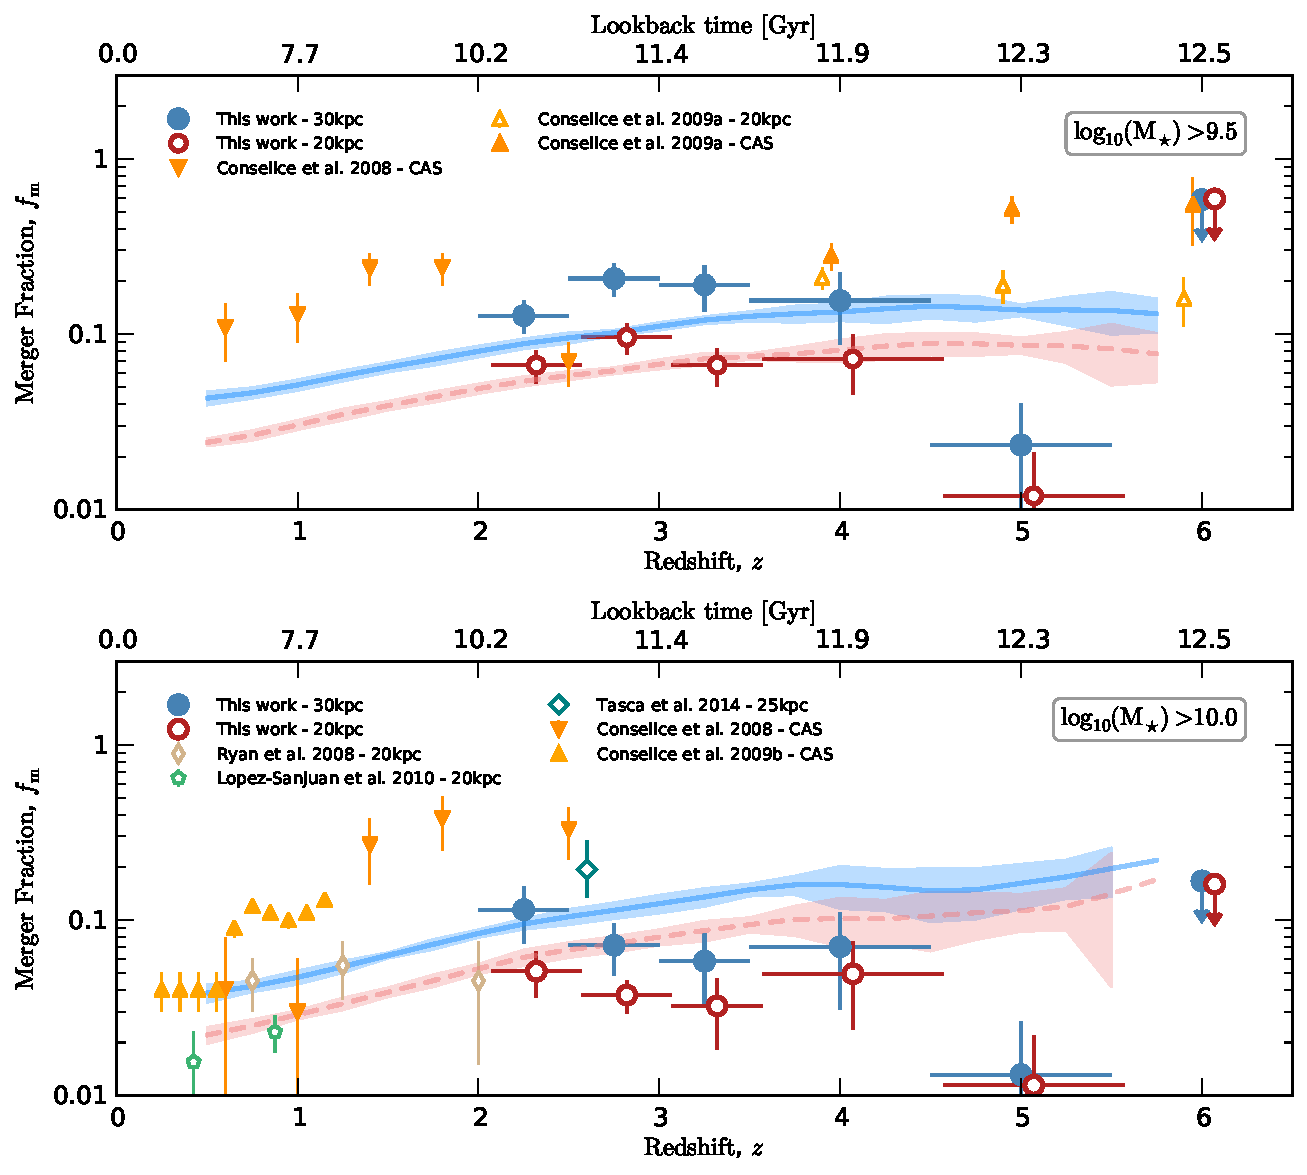
\includegraphics[width=\columnwidth]{plots/merger_fractions.pdf}
  \caption[Estimated merger fraction as a function of redshift.]{Estimated merger fraction as a function of redshift for galaxies with stellar mass $\log_{10}(\Mstar / \text{M}_{\odot}) > 9.5$ (top) and $\log_{10}(\Mstar / \text{M}_{\odot}) > 10$ (bottom). Also shown are the merger fractions from close pair statistics of \citet{RyanJr:2008ka}, \citet{2009MNRAS.397..208C}, \citet{LopezSanjuan:2010cz} and \citet{Tasca:2014gz} and the morphological estimates of \citet{Conselice:2008de},  \citet{2009MNRAS.397..208C} and \citet{Conselice:2009fe}. The continuous blue and dashed red lines correspond to the model predictions of \citet{Lu:2011hj,Lu:2014kl}, with the shaded regions representing the Poisson noise for the model number counts.}
  \label{merger-fig:merger_frac}
\end{figure*}

\begin{table}
  \caption[Estimated merger fractions from PDF analysis, as plotted in Figure~\ref{merger-fig:merger_frac}.]{Estimated merger fractions from PDF analysis, as plotted in Figure~\ref{merger-fig:merger_frac}. Quoted errors include the bootstrapped errors on $f_{\text{m}}$ and the estimated cosmic variance, as calculated in Section~\ref{merger-sec:CV_SAM}.}
\centering
  \begin{tabular}{c|cc}
   \multicolumn{3}{c}{$\text{Merger~fraction}$ - $5 \leq r_{\text{p}} \leq 20$} \\ \noalign{\smallskip}
   Redshift  & $\log_{10}(\Mstar / \text{M}_{\odot}) > 9.5$ & $\log_{10}(\Mstar / \text{M}_{\odot}) > 10$ \\
    \hline
   $2.0 \leq z < 2.5$ & $0.07 \pm 0.02$ & $0.05 \pm 0.02$\\
   $2.5 \leq z < 3.0$ & $0.10 \pm 0.03$&  $0.04 \pm 0.02$\\
   $3.0 \leq z < 3.5$ & $0.07 \pm 0.02$&  $0.03 \pm 0.02$ \\
   $3.5 \leq z < 4.5$ & $0.07 \pm 0.03$&  $0.05 \pm 0.04$\\
   $4.5 \leq z < 5.5$ & $0.01 \pm 0.01$&  $0.01^{+0.02}_{-0.01}$\\
   $5.5 \leq z < 6.5$ & $<  0.59$&  $< 0.16$\\  
    & & \\
    
   \multicolumn{3}{c}{$\text{Merger~fraction}$ - $5 \leq r_{\text{p}} \leq 30$} \\ \noalign{\smallskip}
   Redshift & $\log_{10}(\Mstar / \text{M}_{\odot}) > 9.5$ & $\log_{10}(\Mstar / \text{M}_{\odot}) > 10$ \\
    \hline
   $2.0 \leq z < 2.5$ & $0.13 \pm 0.03$ & $0.11 \pm 0.04$\\
   $2.5 \leq z < 3.0$ & $0.21 \pm 0.04$&  $0.07 \pm 0.04$\\
   $3.0 \leq z < 3.5$ & $0.19 \pm 0.06$&  $0.06 \pm 0.04$ \\
   $3.5 \leq z < 4.5$ & $0.16 \pm 0.07$&  $0.07 \pm 0.04$\\
   $4.5 \leq z < 5.5$ & $0.02 \pm 0.02$&  $0.01^{+0.02}_{-0.01}$\\
   $5.5 \leq z < 6.5$ & $<  0.58$&  $< 0.17$\\  
    
  \end{tabular}\label{tab:fmerger}
\end{table}

We have therefore plotted only those literature results that represent comparable sample selections or methodology. For $\log_{10}(\Mstar / \text{M}_{\odot}) \geq 10$ (bottom panel of Figure~\ref{merger-fig:merger_frac}) we present the close pair results of \citet{RyanJr:2008ka} and \citet{LopezSanjuan:2010cz} at $z\leq2$ and \citet{Tasca:2014gz} at $1.81 \leq z \leq 3.65$. Following \citetalias{LopezSanjuan:2014uj}, since \citet{RyanJr:2008ka} and \citet{LopezSanjuan:2010cz} both present the number of close companions $N_{\rm{c}}$ (i.e. twice the number of close pairs: two galaxies per pair), plotted in Figure~\ref{merger-fig:merger_frac} is $0.5 N_{\rm{c}}$. Also shown are the morphological merger fraction estimates of \citet{Conselice:2008de} and \citet{Conselice:2009fe} at $z \leq 2$. As shown in \citet{Lotz:2008kr} and further discussed in \citet{Bluck:2012dh}, the morphological signatures of mergers are only sensitive to merger ratios of 1:4 or less so are likely probing the same kind of merging systems as is probed by the close pair analysis.

For the $\log_{10}(\Mstar / \text{M}_{\odot}) \geq 9.5$ mass selection (top panel) we show the $9 \leq \log_{10}(\Mstar / \text{M}_{\odot}) \leq 10$ morphology estimates of \citet{Conselice:2008de} and the morphology and pair-count merger rates of \citet{2009MNRAS.397..208C}. Based on a flux limited Lyman break selection, the samples explored by \citet{2009MNRAS.397..208C} likely represent a lower mass range ($\log_{10}(\Mstar / \text{M}_{\odot}) \gtrsim 9$) based on the typical rest-frame magnitude of dropouts in the UDF and the observed mass-to-light ratios at these redshifts Chapter~\ref{ch:smf}. As such, these samples may therefore not represent a valid comparison. 

At $z\sim2$ to 2.5, our results for close pair with projected separations of 20kpc are in good agreement with those of \citet{RyanJr:2008ka} for the same separation and mass limits. However, both results are significantly lower than the morphological estimates of \citet{Conselice:2008de} at this same redshift. Our results currently support the idea that the merger fraction for galaxies with $\log_{10}(\Mstar / \text{M}_{\odot}) \geq 10$ peaks at $z\sim2.5$ \citep{Conselice:2014ct}, with an overall decline in the measured merger fraction above this redshift. However, the fact that the merger fraction declines so sharply at $z\sim5$ is perhaps more likely due to the mass completeness limits applied. As illustrated in Figure~\ref{merger-fig:mass_comp}, for fields with comparable depth to the GOODS Deep or ERS the mass completeness limit is $\log_{10}(\Mstar / \text{M}_{\odot}) \approx 10$. Hence, galaxies which are close to this limit will have fewer companions that are above the completeness limits. The statistical corrections calculated in Section~\ref{merger-sec:weights_flux} rely on having a representative sample of selected companions to up-weight accordingly. Therefore at $z\sim5$ and $z\sim6$ the merger fraction estimates are dominated by the much rarer bright objects in the shallow fields and the very small area of the deeper UDF.

The sharp drop in merger fraction at $z\sim5$ is even more pronounced for the lower mass cut of $\log_{10}(\Mstar / \text{M}_{\odot}) \geq 9.5$, supporting our hypothesis that this drop is driven by issues of mass completeness. The inclusion of the four remaining CANDELS fields may help to reduce this effect by providing more statistically significant samples of galaxies with $\log_{10}(\Mstar / \text{M}_{\odot}) \geq 10$. Furthermore, the increased area covered should provide the number statistics required to investigate the merger fraction at higher mass limits (e.g. $\log_{10}(\Mstar / \text{M}_{\odot}) \geq 10.5$) to better quantify these completeness effects. 

When related to the SAM predictions of \citet{Lu:2011hj}, our estimated merger fractions give rise to somewhat confusing comparisons. For $\log_{10}(\Mstar / \text{M}_{\odot}) \geq 9.5$, the overall evolution and normalisation of the merger fraction at $z\sim2$ to $z\sim4$ are in reasonable agreement with the SAM predictions, especially for pairs selected at 20kpc separation. In contrast the evolution for our observed $f_{\rm{m}}$ at $\log_{10}(\Mstar / \text{M}_{\odot}) \geq 10$ over this same redshift range is markedly different. Interestingly, although the SAM models predict a peak in the merger fractions the redshift at which this occurs is significantly higher than that of earlier observations ($z\sim2.5$; \citeauthor{Conselice:2014ct}~\citeyear{Conselice:2014ct}).

The relatively poor agreement between the observed merger fractions and the results of SAMs for $\log_{10}(\Mstar / \text{M}_{\odot}) \geq 10$ is similar to previous comparisons with models in this way \citep{Bertone:2009jc,Jogee:2009iz}. Typically, SAMs are not necessarily tuned to reproduce observed merger rates at low-redshift \citep{Lu:2014kl}.  As such, it is not necessarily expected that their predicted merger rates match expectations. The observed disagreement is therefore necessarily not indicative of a fault in the observational pair counts.

\subsection{Evolution of the merger rate}\label{merger-sec:mergerrate}
Since the merger fraction itself is a purely observational quantity and not a fundament physical property, it can make comparisons between different redshift bins and methodologies difficult. A more fundamental property of interest is therefore the merger rate, either as the average time between mergers per galaxy ($\Gamma$)\footnote{Referred to in some literature as a merger rate per galaxy \citep{Conselice:2014ct}.} or the overall merger rate, i.e. (specifically the merger rate density, denoted $\mathcal{R}$ in this work).

In order to convert a merger fraction into a merger rate requires knowledge of the merger timescale, $\tau_{\rm{m}}$. The merger timescale can be derived either empirically \citep{Conselice:2009bi} or through simulations \citep{Kitzbichler:2008gi,Lotz:2010ie,Lotz:2010hf}, with different morphology or pair criteria potentially probing different timescales within the merger process. Based on the simulations of \citet{Lotz:2010ie}, we assume merger timescales of $\tau_{\rm{m}} = 0.29$ and $\tau_{\rm{m}} = 0.63$ for pairs with projected separation of $\leq 20$ and $\leq 30$ kpc respectively. These values are based on the average timescales for those separations and similar (baryonic) mass ratios of 1:3. For significantly higher mass ratios of 1:9, the average timescale increases only by $\approx 50\%$, we therefore assume that the relative difference between the 1:3 simulations of \citet{Lotz:2010ie} and the 1:4 ratio's used in this work is minimal. However, the error on the merger timescale for individual simulations can be between $\approx 0.15$ and $>1$ Gyr and the simulations span a range of $\Delta\tau_{\rm{m}} = 0.1$ and 0.38 Gyr for $\leq 20$ and $\leq 30$ kpc respectively. As is the case in all previous studies of the galaxy merger rate, the assumption of merger timescales represents a sizeable systematic uncertainty.

Regardless, the average time between mergers per galaxy is defined simply as
\begin{equation}
	\Gamma(>\Mstar, z) = \frac{\tau_{\text{m}}}{f_{\text{m}}(>\Mstar, z)}
\end{equation}
where $f_{\text{m}}(>\Mstar, z)$ is the merger fraction at redshift $z$ and masses greater than $\Mstar$ (Section~\ref{merger-sec:mergerfraction}) and $\tau_{\text{m}}$ the corresponding merger timescale. Since the timescale is typically of the order of 0.15 to 2+ Gyr, $\Gamma$ is therefore typically quoted in units of Gyr and represents the average timescale between mergers. In Table~\ref{tab:mergerpergal} we present $\Gamma(>\Mstar, z)$ for our estimates of the galaxy merger fraction and the merger timescales outlined above.

If the respective merger timescales for the differing separations (20 kpc and 30 kpc) are accurate, the corresponding merger rates should be the same. For the results of this work, we find that the estimated merger rates per galaxy at $\leq 20$ kpc and $\leq 30$ kpc projected separation are in very good agreement. The fact that the agreement is so good (albeit with very large errors) lends support to the estimated timescales from \citet{Lotz:2010ie}.

Given the estimated time between mergers per galaxy, we can then estimate the relative contribution to the overall stellar mass growth which is a result of mergers. Based on a constant merger rate per galaxy of $\approx 4$ Gyr, a galaxy with $\log_{10}(\Mstar / \text{M}_{\odot}) > 9.5$ will undergo $\approx 0.4$ major mergers in the $\approx 1.7$ Gyr between $z = 4$ and $z=2$. The mass accumulated through major mergers ($\mu = 1/4$) will therefore only contribute an additional $\approx$ 10 to 40\% of the stellar mass in place at $z\sim4$. In contrast, from the observations of Chapter~\ref{ch:smf} we know that galaxies of comparable mass ($\log_{10}(\Mstar / \text{M}_{\odot}) = 9.7 \pm 0.3$) have average specific star-formation rates of $\approx 2.3~\text{Gyr}^{-1}$. Therefore, over the same $\approx 1.7$ Gyr timescale, the in-situ star-formation can increase the galaxy's stellar mass by $\approx 4 \times$. The ratio between the growth by star-formation and growth through \emph{major} mergers is of order $10\times$.

Admittedly, this simple calculation does not take into account the on-going star-formation within the companion galaxy during this same period. For major mergers such as those probed in this study, the star-formation rates within the primary and secondary galaxies in a merging pair will be similar such that the star-formation within the secondary will also be significant. The star-formation rates of galaxies during this epoch are so high that over the assumed merger timescales, the stellar masses of the galaxies within a merger could increase their stellar mass by between $\sim70\%$ and $\sim150\%$ ($\tau_{\text{m}} = 0.29$ and $\tau_{\text{m}} = 0.63$ Gyr respectively).

The rough calculations above do however make two additional assumptions. Firstly, it assumes that the star-formation in both galaxies is not connected, i.e. the on-going star-formation is due to secular evolution. Secondly, that the star-formation duty cycles of both galaxies is long (at least comparable to the merger timescale). However, it is strongly suspected that gas-rich mergers are likely to trigger strong episodes of star-formation within the merging galaxies ('merger triggered starbursts': \citeauthor{Hopkins:2006ju}~\citeyear{Hopkins:2006ju}, \citeauthor{Cox:2008jj}~\citeyear{Cox:2008jj}). The star-formation within galaxies undergoing mergers at high redshift might therefore be significantly enchanced relative to average for galaxies of similar stellar masses. Because the method used in this chapter allows for the identification of galaxies with both high and low pair likelihoods, it is possible to then study the relative star-formation rate properties of those different galaxy populations. In future work we aim to constrain not just the merger rates of galaxies but also the effects those mergers have on star-formation in galaxies over cosmic history.

\begin{table}
  \caption[Average time between mergers for a galaxy in Gyr, $\Gamma$, for the merger fractions presented in Table~\ref{tab:fmerger}.]{Average time between mergers for a galaxy in Gyr, $\Gamma$, for the merger fractions presented in Table~\ref{tab:fmerger}. Assumed timescales are $\tau_{\rm{m}} = 0.29$ Gyr and $\tau_{\rm{m}} = 0.63$ Gyr for projected separations of $5 \leq r_{\text{p}} \leq 20$ kpc and $5 \leq r_{\text{p}} \leq 30$ kpc respectively, see text for details.}
\centering
  \begin{tabular}{c|cc}
   \multicolumn{3}{c}{$\Gamma~[\text{Gyr}]$ - $5 \leq r_{\text{p}} \leq 20$ kpc} \\ \noalign{\smallskip}
   Redshift  & $\log_{10}(\Mstar / \text{M}_{\odot}) > 9.5$ & $\log_{10}(\Mstar / \text{M}_{\odot}) > 10$ \\
    \hline
   $2.0 < z < 2.5$ & $4.4 \pm 1.3$ & $5.7 \pm 2.2$ \\
   $2.5 < z < 3.0$ & $ 3.0 \pm 0.9$ & $7.8 \pm 3.1$\\
   $3.0 < z < 3.5$ & $ 4.4 \pm 1.5$& $ 9.0 \pm 5.4$\\
   $3.5 < z < 4.5$ & $ 4.0 \pm 1.8$& $ 5.9 \pm 4.2$\\
   $4.5 < z < 5.5$ & $ 24.3 \pm 20.5$ & $ 25.5^{+37.3}_{-25.5}$\\
   $5.5 < z < 6.5$ & $ > 0.5$& $> 1.8$ \\  
    & & \\
    
   \multicolumn{3}{c}{$\Gamma~[\text{Gyr}]$ - $5 \leq r_{\text{p}} \leq 30$ kpc} \\ \noalign{\smallskip}
   Redshift & $\log_{10}(\Mstar / \text{M}_{\odot}) > 9.5$ & $\log_{10}(\Mstar / \text{M}_{\odot}) > 10$ \\
    \hline
   $2.0 < z < 2.5$ & $5.0 \pm 1.1$ & $5.6 \pm 2.0$ \\
   $2.5 < z < 3.0$ & $3.1 \pm 0.7$& $8.9 \pm 2.9$\\
   $3.0 < z < 3.5$ & $3.4 \pm 1.0$& $11.0 \pm 4.8$ \\
   $3.5 < z < 4.5$ & $4.1 \pm 1.8$& $9.1 \pm 5.1$\\
   $4.5 < z < 5.5$ & $27.5 \pm 19.8$& $ 48.8^{+64.0}_{-48.4}$\\
   $5.5 < z < 6.5$ & $ > 1.1$ & $>3.8$ \\  
    
  \end{tabular}\label{tab:mergerpergal}
\end{table}


Although more informative than the merger fraction alone, the characteristic time between mergers does not take into account the relative abundances of the galaxies that are merging. We are therefore also interested in the comoving merger rate density, $\mathcal{R}$, defined following \citet{Lin:2004ki} as
\begin{equation}\label{eq:merger_rate}
	\mathcal{R}(>\Mstar, z) = f_{\text{m}}(>\Mstar, z)n_{\text{c}}(\Mstar, z) C_{\rm{m}}\tau_{\text{m}}^{-1},
\end{equation}
where $f_{\text{m}}(>\Mstar, z)$ is the mass and redshift-dependent galaxy merger fraction as above, $n_{\text{c}}(>\Mstar, z)$ the comoving number density for galaxies with stellar mass $>\Mstar$ and $C_{\rm{m}}$ the fraction of galaxies in close pairs that will merge in the timescale $\tau_{\text{m}}$. The comoving number densities for galaxies with $\log_{10}(\Mstar / \text{M}_{\odot}) \geq 9.5$ and $\log_{10}(\Mstar / \text{M}_{\odot}) \geq 10$ are estimated from the same stellar mass function parametrisations used for the mass completeness weights. Specifically, those of \citet{Mortlock:2014et} at $z \leq 3$, \citet{Santini:2012jq} at $3 < z < 3.5$ and from Chapter~\ref{ch:smf} at $z \geq 3.5$. Errors on the number densities are estimated by perturbing the Schechter function parameters based on their quoted errors and recalculating the integrated number density. This step is then repeated 1000 times and the lower and upper 1-$\sigma$ errors are taken as the \nth{16} and \nth{84} percentiles.

\begin{figure*}
\centering
	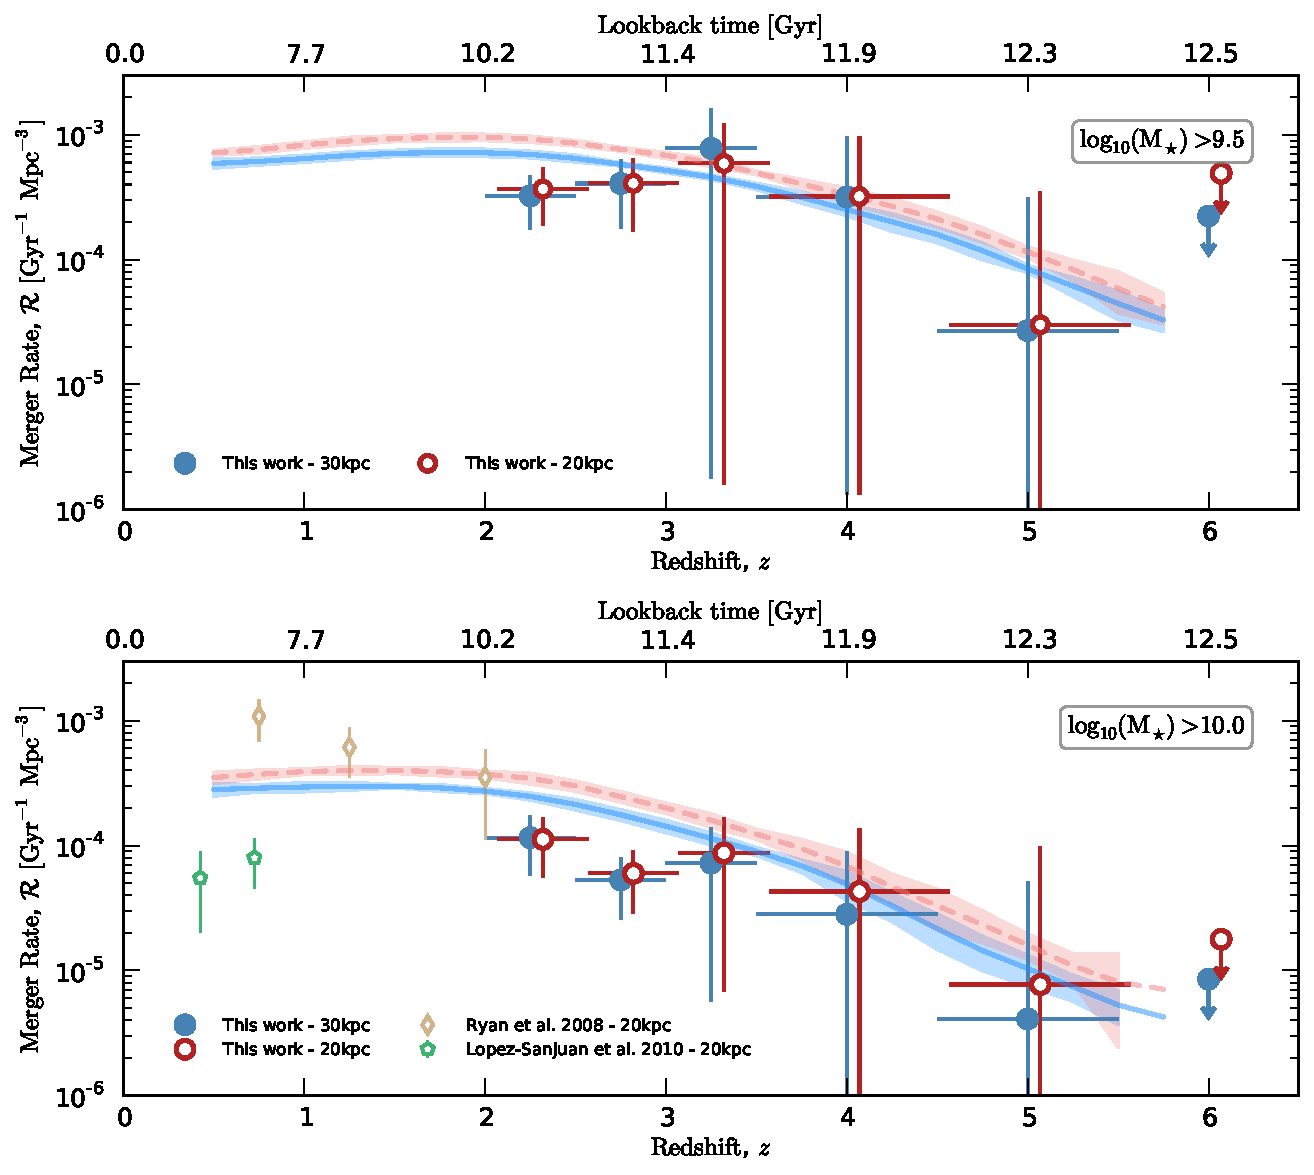
\includegraphics[width=\columnwidth]{plots/merger_rate.pdf}
  \caption[Estimated galaxy merger rates as a function of redshift.]{Estimated galaxy merger rates as a function of redshift for galaxies with stellar mass $\log_{10}(\Mstar / \text{M}_{\odot}) > 9.5$ (top) and $\log_{10}(\Mstar / \text{M}_{\odot}) > 10$ (bottom). The merger rates are calculated following Equation~\ref{eq:merger_rate}, assuming $\tau_{\rm{m}} = 0.29$ and $0.64$ Gyr for the 20 and 30kpc estimates respectively.   Also shown are the merger rates from close pair statistics of \citet{RyanJr:2008ka} and \citet{LopezSanjuan:2010cz}. The continuous blue and dashed red lines correspond to the model predictions of \citet{Lu:2011hj,Lu:2014kl}, with the shaded regions representing the Poisson noise for the model number counts.}
  \label{merger-fig:merger_rate}
\end{figure*}

In Figure~\ref{merger-fig:merger_rate} we show the resulting merger rate densities calculated following Equation~\ref{eq:merger_rate}. Plotted are the merger fractions estimated in this work and the model predictions of \citet{Lu:2011hj} for which the comoving number densities have been calculated directly from the models (Lu, \emph{priv. communication}). We also plot the merger rates quoted by \citet{LopezSanjuan:2010cz} and the merger density values of \citet{RyanJr:2008ka} converted to merger rates using the same timescale ($\tau_{\rm{m}} = 0.29$) as used for the 20kpc estimates of this work. The estimated merger rates and corresponding errors are also shown in Table~\ref{tab:merger_rate_dens}. It is worth noting that the large uncertainty at the high-mass end of the stellar mass function results in significantly larger errors for the merger rates than the corresponding estimates for the merger fraction.

For $\log_{10}(\Mstar / \text{M}_{\odot}) > 10$, the merger rate gradually declines beyond $z\geq 2$, with the discrepancy between $z\sim4$ and $z\sim5$ less stark. For the merger rate of galaxies with $\log_{10}(\Mstar / \text{M}_{\odot}) > 9.5$, over the whole redshift range studied in this work the merger rate also declines and is roughly consistent with the predictions of \citet{Lu:2011hj}. However, for both mass selections, when the mass completeness affected $z\sim5$ observations are discounted the remaining observations are consistent with remaining constant between $2 \lesssim z \lesssim 4$. Given the large errors in the current observations, it is clearly difficult to draw any meaningful conclusions about the redshift evolution of the merger fraction at $z > 3$.
  
When compared to the literature values of \citet{RyanJr:2008ka} at $z\sim2$, the merger rate density measured in this work is significantly lower at $z\sim 2.25$ (by a factor of $\approx 3\times$). Given the good agreement in the merger fractions and the identical assumed merger timescales, this discrepancy is likely due to a difference in the assumed comoving number densities. We have excluded the results of \citet{2009MNRAS.397..208C} at $z\geq 4$ in Figure~\ref{merger-fig:merger_rate} as the Lyman break selection used in that analysis make it difficult to retrospectively estimate accurate corresponding comoving number densities for the samples studied.

For the comoving merger rates predicted by the semi-analytic models, there is a small disagreement between the $\leq 20$ kpc and $\leq 30$ kpc close pair estimates with those for $\leq 20$ kpc being $\approx 30\%$ higher. Given the large systematic uncertainty (and variation) in the merger timescales \citep{Lotz:2008kr,Lotz:2010hf,Lotz:2010ie} this to be expected when a simplified average is used. A critical goal for future work is therefore to estimate the true merger rate within the models (i.e. directly from the merger trees) in order to test the origin of this difference and further explore the scatter and evolution of the predicted merger timescales at $z\geq 2$.

\begin{table}
  \caption[Comoving merger rate, $\mathcal{R}$ in units of $10^{-4}~\text{Gyr}^{-1}~\text{Mpc}^{-3}$ for the merger fractions presented in Table~\ref{tab:fmerger}.]{Comoving merger rate, $\mathcal{R}$ in units of $10^{-4}~\text{Gyr}^{-1}~\text{Mpc}^{-3}$ for the merger fractions presented in Table~\ref{tab:fmerger}. Assumed timescales are $\tau_{\rm{m}} = 0.29$ and  $0.63$ Gyr for projected separations of $5 \leq r_{\text{p}} \leq 20$ kpc and $5 \leq r_{\text{p}} \leq 30$ kpc respectively, see text for further details. Comoving number densities for the mass selected samples are calculated from the corresponding stellar mass functions as described in the text.}
\centering
  \begin{tabular}{c|cc}
   \multicolumn{3}{c}{$\text{Merger~rate,}~\mathcal{R}~[10^{-4}~\text{Gyr}^{-1}~\text{Mpc}^{-3}]$ - $5 \leq r_{\text{p}} \leq 20$ kpc} \\ \noalign{\smallskip}
   Redshift  & $\log_{10}(\Mstar / \text{M}_{\odot}) > 9.5$ & $\log_{10}(\Mstar / \text{M}_{\odot}) > 10$ \\
    \hline
   $2.0 < z < 2.5$ & $3.64 \pm 1.83$ & $3.22 \pm 1.51$ \\
   $2.5 < z < 3.0$ & $4.21 \pm 2.28$ & $4.20 \pm 2.18$\\
   $3.0 < z < 3.5$ & $5.36^{+6.36}_{-5.36}$& $7.07^{+8.30}_{-7.07}$ \\
   $3.5 < z < 4.5$ & $3.18^{+6.61}_{-3.18}$& $3.15^{+6.55}_{-3.15}$ \\
   $4.5 < z < 5.5$ & $0.28^{+4.07}_{-0.28}$& $0.25^{+3.65}_{-0.25}$ \\
   $5.5 < z < 6.5$ & $<3.76$& $<1.71$\\  
    & & \\
    
   \multicolumn{3}{c}{$\text{Merger~rate,}~\mathcal{R}~[10^{-4}~\text{Gyr}^{-1}~\text{Mpc}^{-3}]$ - $5 \leq r_{\text{p}} \leq 30$ kpc} \\ \noalign{\smallskip}
   Redshift & $\log_{10}(\Mstar / \text{M}_{\odot}) > 9.5$ & $\log_{10}(\Mstar / \text{M}_{\odot}) > 10$ \\
    \hline
   $2.0 < z < 2.5$ & $1.11 \pm 0.55$ & $1.15 \pm 0.57$ \\
   $2.5 < z < 3.0$ & $0.58 \pm 0.31$ & $0.52 \pm 0.28$\\
   $3.0 < z < 3.5$ & $0.85 \pm 0.83$ & $0.70 \pm 0.69$ \\
   $3.5 < z < 4.5$ & $0.43^{+1.03}_{-0.43}$& $0.28^{+0.68}_{-0.28}$ \\
   $4.5 < z < 5.5$ & $0.07^{+0.82}_{-0.07}$& $0.04^{+0.43}_{-0.04}$ \\
   $5.5 < z < 6.5$ & $<0.18$ & $<0.09$\\  
    
  \end{tabular}\label{tab:merger_rate_dens}
\end{table}

\subsection{Minor mergers}\label{merger-sec:minor}
The merger fraction and corresponding merger rate results presented in this section have been for major mergers only (defined as $\mu \geq 1/4$). This choice was primarily motivated by the expected limits on the mass completeness at the high redshift we aimed to probe, as the mass of secondary galaxies in mergers with mass ratios $>4$ will typically be significantly below the mass completeness limits and thus excluded from our analysis. However, based on the estimated mass completeness levels at $z \leq 3$ in Figure~\ref{merger-fig:mass_comp}, the deep CANDELS GOODS South data will clearly allow for merger fraction estimates for mass ratios up to $\geq 10$ for mass selections $\log_{10}(\Mstar / \text{M}_{\odot}) > 10$ and even higher for more massive samples. This wide dynamic range will should make it possible to measure the merger rate as a function of $\mu$ in future work, fully quantifying the relative contribution of mergers at different mass ratios over a crucial period in the evolution of galaxies (e.g. \citeauthor{Bluck:2012dh}~\citeyear{Bluck:2012dh}).

Based on the observed galaxy stellar mass function evolution, to first order we would expect the relative number of minor to major mergers to be greater at high redshift (for a galaxy of a given mass, the relative number of lower mass galaxies will be higher for steeper mass functions). The relative contribution of minor mergers to the stellar mass growth of massive galaxies should therefore also be greater at high redshift. For the most massive galaxies at $z \leq 3$, \citet{Ownsworth:2014gt} estimated the inverse to be true; with the ratio of minor to major merger fuelled growth found to be \emph{decreasing} with increasing redshift (see also \citeauthor{Bluck:2012dh}~\citeyear{Bluck:2012dh}). Even if minor mergers make only a minor contribution to the overall stellar mass growth of galaxies below $z = 3$, they are still expected to have a significant effect on the size growth of massive galaxies \citep{Trujillo:2011jy,Newman:2012hp,McLure:2012hq} during this period. Understanding how the relative contributions from different merger ratios change will provide extremely useful clues as to what processes are driving the evolution of the galaxy stellar mass function in this epoch.

\section{Discussion}\label{merger-sec:discussion}
In the results presented in Section~\ref{merger-sec:results} we have shown that using the probabilistic redshift PDF pair-count method it is possible to obtain estimates of the merger fraction out to redshifts of $z\sim4$ and potentially beyond. The major drawback based on these early results is down to the compounding effects of increasing mass incompleteness with redshift and the rapidly decreasing number density of massive galaxies at higher redshift \citep{Duncan:2014gh,Grazian:2014vx}. 

Despite the large uncertainties, our results give us cause for optimism with regards to studying merger rates at $z \geq 2$ and into the first billion years of galaxy evolution. The inclusion of the additional 4 remaining CANDELS fields will help to reduce the existing uncertainties by significantly increasing the volume being probed and reducing the error from cosmic variance. Of particular interest will be the GOODS North field. Firstly, it will double the area of CANDELS DEEP data being studied, improving the small samples of the faint highest redshift galaxies. Secondly this field benefits from the very deep SHARDS narrowband survey \citep{PerezGonzalez:2012fo}, allowing for significantly improved photometric redshift accuracy. The additional larger WIDE fields of COSMOS, EGS and UDS will also be ideal for selecting the rarer high-mass galaxies at $z\sim5$ and $z\sim6$ required to improve the estimates available from GOODS South alone. Finally, the Frontier Fields parallels \citep{2015ApJ...800...84C} will provide deep HST photometry for 6 additional blank fields with depths comparable to those of the Hubble Ultra-deep Field. These additional fields will be vital for further increasing the available samples of galaxies at $z \geq 5$.

If gas-rich major mergers play a critical role in driving AGN accretion and quasar activity \citep{Springel:2005co,Hopkins:2008gr}, linking the evolution of galaxy merger rates and AGN activity through cosmic history is clearly of key importance. Based on the declining merger rates calculated in this work, there is certainly no strong evidence against a correlation between the quasar or AGN luminosity density and the merger rate density. Given the preliminary nature of these results and the scarcity of directly comparable merger rate estimates at $z < 2$ (i.e. in mass selection) we are wary of trying to parametrise our results for such a comparison. As discussed in \citet{Conselice:2014ct}, parametrisations of the merger history at $z < 3$ can be systematically affected by the very low redshift ($z\sim0$) anchor point. 

However, such an analysis will soon be much more viable. In combination with a forthcoming study of galaxy merger fractions at $z < 3$ in the deep ground-based fields of UltraVISTA \citep{McCracken:2012gd}, UDS \citep{Lawrence:2007hu} and VIDEO \citep{Jarvis:2012hr} (Mundy et al. \emph{in prep}), the close pair merger analysis of CANDELS will make it possible to study the full assembly of massive galaxies over almost the complete cosmic history.

With the improved merger fraction estimates measured for the full CANDELS dataset, it is likely that the limiting uncertainty on the fundamental physical properties such as the merger rate density will actually be the merger timescales and the constraints on the true number densities of the samples of interest. As well as reducing the statistical uncertainties in the merger fraction estimates, the wealth of additional ground and space-based data available will be crucial in providing better constraints on the galaxy stellar mass function at high redshifts. 

With the new generation of hydrodynamical simulations over cosmological volumes (e.g. Illustris, \citeauthor{Vogelsberger:2014gw}~\citeyear{Vogelsberger:2014gw}; EAGLE, \citeauthor{Schaye:2014gk}~\citeyear{Schaye:2014gk}), it is also now possible to study the variation and evolution of merger timescales for large samples of mergers. Not only will representative sample of galaxy properties and environments provide key insights into the the systematic variation of merger timescales, the ability to perform identical analyses to synthetic images of these simulations \citep{Torrey:2015kx} will greatly improve our understanding of the systematics errors and biases involved.

\section{Summary}\label{merger-sec:summary}
In this chapter we have estimated the major merger fraction of galaxies at $z\geq 2$ in the CANDELS GOODS South field \citep{Guo:2013ig} by analysing the close pair statistics. The close pair method used is based on that presented by \citet{LopezSanjuan:2014uj} and makes use of the full photometric redshift probability distribution to account for line-of-sight separation in the absence of high-quality spectroscopic data.

The merger fractions based on close pairs were measured for projected separations of $5 \leq r_{\text{p}} \leq 20$ kpc and $5 \leq r_{\text{p}} \leq 30$ kpc. For a mass selection of $\log_{10}(\Mstar / \text{M}_{\odot}) > 9.5$ and merger ratios of 1:4 or less ($\mu > 1/4$) the merger fraction  is approximately constant between $z \approx 2.25$ and $z\sim4$ with a potential peak at $z\approx3$. Similarly, for a mass selection of $\log_{10}(\Mstar / \text{M}_{\odot}) > 10$ the merger fraction is consistent with constant or in slight decline of this same redshift range. For both mass selections the observed merger fraction rapidly declines at $z\sim5$, something which we believe is most likely due to the effects of the mass-completeness limit applied to the analysis. Future work over wider survey areas should produce more statistically significant high mass samples at these redshifts and allow us to better investigate the nature of this drop.

Assuming merger timescales from simulations of \citet{Lotz:2010ie}, we estimate the average time between mergers per galaxy ($\Gamma$, in Gyr) and the comoving merger rate density ($\mathcal{R}$, $\text{Gyr}^{-1} ~ \text{Mpc}^{-3}$) for our observed merger fractions. The estimated $\Gamma$ at $2 \lesssim z \lesssim 4$ (where our merger fractions are reasonably well constrained) are consistent with a constant $\approx 4 ~\text{Gyr}$ for $\log_{10}(\Mstar / \text{M}_{\odot}) > 9.5$ and $\approx 8 ~\text{Gyr}$ for $\log_{10}(\Mstar / \text{M}_{\odot}) > 9.5$. Relative to the on-going star-formation within galaxies over this redshift range, this low merger rate means that the galaxy growth through star-formation is of order $10\times$ greater than the growth through major mergers.

For both mass selections, the estimated comoving merger rate density, $\mathcal{R}$, gradually declines at $z\geq 2$. However, due to the large uncertainties in the high-mass end of the galaxy stellar mass function (and hence the estimated number densities) the errors on $\mathcal{R}$ are too large to draw any meaningful conclusions with regards to the mechanisms of galaxy assembly.

Given the limited dataset on which we have tested the redshift PDF merger methodology, we are confident that many of the existing uncertainties can be greatly reduced with the inclusion and analysis of existing available data. With careful analysis, it should soon be possible to build an observational picture of the assembly history of mass galaxies.



